%% Week 47 -- Boosting: AdaBoost, steepest descent in function space,
%% gradient boosting and XGBoost (Chapter 7, Sections 7.11-7.16).  Monday
%% lecture, 2 x 45 min.  Part 1: a short repetition of bagging and random
%% forests and why we use ensembles at all (7.8-7.10, Eq. 7.16).  Part 2:
%% boosting from a bird's eye view -- additive models, forward stagewise
%% fitting, a toy example worked out (7.11).  Part 3: AdaBoost -- the
%% algorithm, a first round by hand, where it comes from (the exponential
%% loss), what it estimates, margins (7.12).  Part 4: our own AdaBoost against
%% scikit-learn on the moons.  Part 5: steepest descent in function space and
%% why the literal version is useless (7.13).  Part 6: gradient boosting with
%% scikit-learn: regression, shrinkage, classification (7.13).  Part 7:
%% XGBoost -- second-order objective, the closed-form leaf weights, the gain,
%% regularization, the cancer data (7.14).  Part 8: summary, a pointer to
%% 7.15, and the plan for the last two weeks.
%% Figures: week47_*.pdf from make_week47_figures.py, plus week46_variance,
%% week46_ensembles and week46_cancer from make_week46_figures.py for the
%% recap.  Companion notebook: week47.ipynb.
%% Book references (book.aux 2026-10-25): Sections 7.11-7.16; Eqs 7.14-7.16
%% (variance of an average), 7.19 (additive model), 7.20 (stagewise), 7.21
%% (error rate), 7.22 (AdaBoost combination), 7.23 (exponential loss), 7.24
%% (weights), 7.25 (split of the criterion), 7.26 (weighted error), 7.27
%% (beta_m), 7.28 (weight update), 7.29 (alpha_m), 7.30 (functional
%% gradient), 7.31 (GB squared loss), 7.32 (GB logistic), 7.33 (XGB
%% objective), 7.34 (penalty), 7.35 (per-leaf form), 7.36 (leaf weight and
%% score), 7.37 (gain), 7.38 (gain for the squared error); Fig. 7.4.
%% Build:  pdflatex week47slides.tex  (twice)
\documentclass[10pt,aspectratio=169]{beamer}
\usetheme{red_plain}
\usepackage[T1]{fontenc}
\usepackage[utf8]{inputenc}
\usepackage{amsmath,amssymb,bm}
\usepackage{graphicx}
\usepackage{listings}
\usepackage{xcolor}
\usepackage{booktabs}
\graphicspath{{../BookFigures/chapter07_trees_and_ensembles/}{./ch7/}{./}}

%% ---- code listings
\definecolor{codebg}{rgb}{0.97,0.97,0.97}
\lstset{language=Python,basicstyle=\ttfamily\scriptsize,backgroundcolor=\color{codebg},
  keywordstyle=\color{blue!70!black}\bfseries,commentstyle=\color{green!45!black},
  stringstyle=\color{red!60!black},showstringspaces=false,frame=single,
  framerule=0pt,xleftmargin=4pt,xrightmargin=4pt,breaklines=true,columns=fullflexible}

%% ---- the "pause and think" question frames
\newcounter{insight}
\newenvironment{insight}[1][]{%
  \stepcounter{insight}%
  \begin{frame}{Pause and think \arabic{insight}: #1}%
  \setbeamercolor{block title}{bg=structure.fg,fg=white}%
  \setbeamercolor{block body}{bg=structure.fg!8}%
  \small
}{\end{frame}}
\newcommand{\question}[1]{\begin{block}{Question}#1\end{block}}
\newcommand{\answer}[1]{\pause\begin{block}{Answer}#1\end{block}}

\setbeamertemplate{footline}[frame number]
\setbeamerfont{block title}{size=\small}
\setbeamertemplate{blocks}[rounded][shadow=false]
\setbeamercovered{invisible}

\newcommand{\var}{\mathrm{var}}
\newcommand{\cov}{\mathrm{cov}}
\newcommand{\err}{\overline{\mathrm{err}}}
\newcommand{\sgn}{\mathrm{sign}}

\title{Week 47: Boosting}
\subtitle{From bagging to boosting -- AdaBoost by hand and from scratch,
  steepest descent in function space, gradient boosting with
  \texttt{scikit-learn}, and XGBoost}
\author{Morten Hjorth-Jensen}
\institute{Department of Physics and Center for Computing in Science Education,\\
  University of Oslo, Norway}
\date{}

\begin{document}

\begin{frame}
\titlepage
\end{frame}

\begin{frame}{Plan for week 47}
\footnotesize
\textbf{Monday lecture (2$\times$45 min): Chapter 7, Sections 7.11--7.16.}
\begin{enumerate}
  \item \textbf{Repetition}: why ensembles at all -- the variance of a tree,
    Eq.\ (7.16), bagging and random forests, and what they cannot do.
  \item \textbf{Boosting from a bird's eye view} (7.11): additive models,
    forward stagewise fitting, a toy example worked out by hand.
  \item \textbf{AdaBoost} (7.12): the algorithm, a first round by hand, where
    the strange formulas come from (the exponential loss), what the
    classifier estimates, margins.
  \item \textbf{Our own AdaBoost against \texttt{scikit-learn}}: weighted
    trees, the class of Section 7.12, the moons.
  \item \textbf{Steepest descent in function space} (7.13): the gradient of a
    loss with respect to the predictions, why the literal algorithm is
    useless, and how a tree repairs it.
  \item \textbf{Gradient boosting} with \texttt{scikit-learn}: regression,
    shrinkage against the number of trees, classification with the logistic
    loss.
  \item \textbf{XGBoost} (7.14): second-order objective, the closed-form leaf
    weights, the gain, $\lambda$ and $\gamma$, the cancer data.
  \item \textbf{Summary} and the plan for weeks 47--48.
\end{enumerate}
\textbf{Tuesday (flipped classroom, the last one)}: your Project-3 proposal
presentations, 3--5 slides and 3--5 minutes per group.  The slides are the
week-47 exercise, due Friday November 20.

\textbf{Reading}: Sections 7.11--7.16; Hastie, Tibshirani and Friedman
Chapter 10; Chen and Guestrin, \emph{XGBoost: A Scalable Tree Boosting
System} (2016).  Code: \texttt{week47.ipynb}, \texttt{make\_week47\_figures.py}.
\end{frame}

%% =====================================================================
\section{Repetition: why ensembles?}
%% =====================================================================

\begin{frame}{Where we were: a single tree is a high-variance estimator}
\begin{columns}[T]
\begin{column}{0.52\textwidth}
\small
Last week we grew a tree by recursive binary splitting and found it
\textbf{readable, fast, scale-free} -- and \textbf{unstable}.  The reason was
quantitative (week 46, ``why a tree has high variance''):
\begin{itemize}
  \item a leaf with $n_m$ points predicts their mean, with variance
    $\sigma^2/n_m$; a fully grown tree has $n_m=1$ and reproduces the noise,
    expected test error $2\sigma^2$ -- twice the irreducible error;
  \item a shallow tree has small variance but large bias: a piecewise
    constant with few pieces;
  \item on top of that the \emph{partition itself} is random -- a slightly
    different training set moves the cutpoints, and by the law of total
    variance that adds a second term.
\end{itemize}
On the noisy Runge function: depth-4 tree $0.0181$, full tree $0.0214$,
a degree-10 polynomial $0.0133$, noise floor $0.0100$.
\end{column}
\begin{column}{0.46\textwidth}
\begin{block}{The two ways out}
\small
\textbf{Average} many high-variance, low-bias trees so the noise cancels
(bagging, random forests -- last week), or \textbf{add up} many low-variance,
high-bias trees so the bias cancels (boosting -- today).  Both build
\[
f(\bm{x})=\sum_{m=1}^M \beta_m\, T_m(\bm{x}),
\]
and the whole difference is in how the $T_m$ and the $\beta_m$ are chosen:
independently and in parallel, or one after the other, each correcting the
last.
\end{block}
\end{column}
\end{columns}
\end{frame}

\begin{frame}{Repetition 1: the variance of an average, Eq.\ (7.16)}
\begin{columns}[T]
\begin{column}{0.5\textwidth}
\small
$B$ estimators $f_1,\dots,f_B$, each with variance $\sigma^2$, pairwise
correlation $\rho$.  Their average $\bar f=\frac1B\sum_b f_b$ has
\[
\var(\bar f)=\frac{1}{B^2}\Big[\sum_b\var(f_b)+\sum_{b\neq b'}\cov(f_b,f_{b'})\Big]
\]
\[
\phantom{\var(\bar f)}=\frac{\sigma^2}{B}+\frac{B(B-1)}{B^2}\rho\sigma^2
=\rho\sigma^2+\frac{1-\rho}{B}\sigma^2 .
\]
\begin{itemize}
  \item independent members ($\rho=0$): variance $\sigma^2/B$, Eq.\ (7.14);
  \item correlated members: the second term dies with $B$, the \textbf{floor
    $\rho\sigma^2$ does not};
  \item averaging never changes the \textbf{expectation}: $\mathbb{E}\bar
    f=\mathbb{E}f_b$.  The bias of the members is the bias of the average.
\end{itemize}
\end{column}
\begin{column}{0.5\textwidth}
\small
\textbf{Bagging} (Section 7.9): $B$ bootstrap samples, one deep tree on
each, average (regression) or majority vote (classification).  The
out-of-bag points of each tree give a free test set, Eq.\ (7.17).

\textbf{Random forests} (Section 7.10): the same, but at every split only
$m\approx\sqrt p$ random features are candidates, Eq.\ (7.18).  Bagged trees
of the same data all split on the same strong feature first and are
correlated; restricting the candidates \textbf{lowers $\rho$} and therefore
the floor.

Measured last week on the Runge data: $\sigma^2=0.0102$ for one tree,
$\rho=0.46$ between two bagged trees -- averaging a hundred of them removes
about half the variance and then stops.  On the cancer data $\rho$ fell from
$0.81$ (bagging) to $0.78$ (forest, $m=5$).
\end{column}
\end{columns}
\end{frame}

\begin{frame}{Repetition 2: Eq.\ (7.16) measured, and the ensembles on the moons}
\centering
\includegraphics[width=0.98\textwidth]{week46_variance.pdf}\\
\small
\textbf{Left}: $\var(\bar f)/\sigma^2$ against $B$ for several $\rho$;
dotted lines are the floors.  \textbf{Middle}: 200 independent training sets
of the noisy Runge function, 100 bagged trees on each -- the measured
variance of the average follows the formula with the measured $\sigma^2$ and
$\rho$ and no fitting.  \textbf{Right}: Condorcet's jury -- $B$ independent
voters each right with probability $p>1/2$ become a strong majority.  The
italics are the assumption that bagging only approximately satisfies, and
that boosting will replace by a different mechanism altogether.
\end{frame}

\begin{frame}{Repetition 3: what we got on the data sets, and what we did not get}
\begin{columns}[T]
\begin{column}{0.5\textwidth}
\small
\textbf{Moons} ($n=500$, noise $0.3$, 375/125 split): single tree $0.824$,
bagging $0.907$ ($0.923$ in \texttt{scikit-learn}), random forest $0.909$
($0.915$).

\textbf{Breast cancer} ($569\times30$, 398/171 split): tree of depth 3
$0.918$, full tree $0.930$, bagging $0.942$, random forest $0.953$ --
\textbf{logistic regression $0.965$}.

The islands around single points were averaged away, the boundary became
smooth and came with a graded confidence (the fraction of votes).  The gain
was complete by $B\approx50$.
\end{column}
\begin{column}{0.5\textwidth}
\begin{block}{What averaging cannot do}
\small
\begin{itemize}
  \item It cannot remove the \textbf{bias} of its members.  A forest of
    stumps (depth 1) is still additive in the features: no averaging makes
    it learn an interaction.
  \item It cannot do better than \textbf{the floor} $\rho\sigma^2$.
  \item It treats every training point the same at every step; a point every
    tree gets wrong stays wrong.
\end{itemize}
Boosting fixes all three by \textbf{building the members sequentially}: each
new one is fitted to what the previous ones got wrong.  The members can then
be very simple -- \emph{weak learners} -- and the bias is reduced step by
step.
\end{block}
\end{column}
\end{columns}
\end{frame}

\begin{insight}[can bagging ever beat the bias of its members?]
\question{We bag $B=10^6$ decision \emph{stumps} (one split each) on data
with a target $y=x_1x_2+\epsilon$, $x_1,x_2\in\{-1,+1\}$.  Does the
bagged prediction converge to the truth as $B\to\infty$?  What does the
same question look like for boosting?}
\answer{No.  A stump is a function of one feature, so every member is of the
form $g(x_1)$ or $h(x_2)$, and so is any average of them -- an additive
function $a(x_1)+b(x_2)$.  But $x_1x_2$ is orthogonal to every additive
function on this domain (sum over the four corners), so the best additive
approximation is the constant $0$: the bagged prediction converges, with
probability one, to a function with \textbf{zero correlation with the
target}.  Averaging removes the variance $\sigma^2(1-\rho)/B$, not the bias.
Boosting stumps gives the same additive class, so it fails here too -- but
boosting trees of depth 2 can represent $x_1x_2$ exactly: the depth of the
weak learner sets the \textbf{interaction order} of the model, one of the
few knobs that matter.}
\end{insight}

%% =====================================================================
\section{Boosting from a bird's eye view (Section 7.11)}
%% =====================================================================

\begin{frame}{Boosting from a bird's eye view: additive models fitted forward}
\begin{columns}[T]
\begin{column}{0.52\textwidth}
\footnotesize
Boosting fits an \textbf{additive expansion} in a set of simple basis
functions $b(\bm{x};\gamma)$ -- stumps, small trees, splines, anything with a
few parameters $\gamma$:
\[
f_M(\bm{x})=\sum_{m=1}^M\beta_m\,b(\bm{x};\gamma_m).\tag{7.19}
\]
Fitting all $(\beta_m,\gamma_m)$ at once,
\[
\min_{\{\beta_m,\gamma_m\}}\sum_{i=1}^n L\Big(y_i,\sum_m\beta_m b(\bm{x}_i;\gamma_m)\Big),
\]
is hopeless for trees.  \textbf{Forward stagewise} fitting instead adds one
term at a time and never revisits the old ones:
\[
(\beta_m,\gamma_m)=\arg\min_{\beta,\gamma}\sum_{i=1}^n
L\big(y_i,\,f_{m-1}(\bm{x}_i)+\beta\, b(\bm{x}_i;\gamma)\big),\tag{7.20}
\]
\[
f_m(\bm{x})=f_{m-1}(\bm{x})+\beta_m b(\bm{x};\gamma_m),\qquad f_0=0 .
\]
\end{column}
\begin{column}{0.46\textwidth}
\begin{block}{Three ideas in one line}
\footnotesize
\begin{enumerate}
  \item \textbf{Weak learners}: $b$ is simple, slightly better than guessing.
  \item \textbf{Sequential}: term $m$ sees the residual of terms $1..m-1$,
    so it concentrates on what is still wrong -- in AdaBoost through
    \emph{weights} on the points, in gradient boosting through
    \emph{pseudo-residuals}.
  \item \textbf{Greedy}: each $(\beta_m,\gamma_m)$ is optimal given the past
    and frozen afterwards.  Slow, but it works -- and the slowness turns out
    to be a form of regularization.
\end{enumerate}
\end{block}
\footnotesize
The whole lecture is Eq.\ (7.20) for three choices of the loss $L$ and of the
weak learner $b$: the exponential loss and stumps (AdaBoost), any
differentiable loss and regression trees (gradient boosting), and a
second-order expansion of any loss with regularized trees (XGBoost).
\end{column}
\end{columns}
\end{frame}

\begin{frame}{A toy case worked out: $b(x;\gamma)=1+\gamma x$ and the squared error}
\begin{columns}[T]
\begin{column}{0.54\textwidth}
\footnotesize
Take one feature, $L(y,f)=(y-f)^2$ and the two-parameter basis function
$b(x;\gamma)=1+\gamma x$.  One stage of Eq.\ (7.20) with residual vector
$\bm{r}=\bm{y}-f_{m-1}(\bm{x})$ is
\[
\min_{\beta,\gamma}\;\big\|\bm{r}-\beta(\bm{e}+\gamma\bm{x})\big\|^2,
\qquad \bm{e}=(1,\dots,1)^T .
\]
Write $\bm{w}=\bm{e}+\gamma\bm{x}$.  For fixed $\gamma$ the problem in
$\beta$ is ordinary least squares with one column,
\[
\beta=\frac{\bm{w}^T\bm{r}}{\bm{w}^T\bm{w}} .
\]
For fixed $\beta$, $\partial/\partial\gamma$ of the sum of squares gives
$\bm{x}^T(\bm{r}-\beta\bm{e}-\beta\gamma\bm{x})=0$, that is
\[
\gamma=\frac{\bm{x}^T\bm{r}-\beta\,\bm{x}^T\bm{e}}{\beta\,\bm{x}^T\bm{x}} .
\]
Alternate the two until they stop moving: an inner \textbf{iterative fit}
of the basis function, then the outer stagewise step
$f_m=f_{m-1}+\beta(1+\gamma x)$, then the next residual.
\end{column}
\begin{column}{0.44\textwidth}
\begin{block}{What to take from the toy}
\footnotesize
\begin{itemize}
  \item A basis function with a nonlinear parameter ($\gamma$ inside $b$)
    needs an inner optimization; for a tree, $\gamma$ is the set of splits and
    leaf values and the inner optimization is \textbf{CART itself}.
  \item Only the \textbf{residual} enters stage $m$.  The squared error makes
    this literal; other losses replace the residual by a generalized one (the
    negative gradient, Section 7.13).
  \item Nothing forces $\beta_m$ to be the exact minimizer -- shrinking it,
    $f_m=f_{m-1}+\nu\beta_m b$, $0<\nu<1$, costs more stages and buys
    stability.  All libraries do this.
\end{itemize}
\end{block}
\end{column}
\end{columns}
\end{frame}

\begin{frame}{Weak learners}
\footnotesize
\begin{columns}[T]
\begin{column}{0.5\textwidth}
A \textbf{weak learner} for two classes is any rule with error rate
\[
\err=\frac1n\sum_{i=1}^n I(y_i\neq G(\bm{x}_i))<\tfrac12 ,\tag{7.21}
\]
strictly better than a coin -- a \textbf{decision stump} (a tree with one
split, so the classifier is a threshold on one feature) is the canonical
example.  Stumps alone are poor: on the moons a single stump gets $0.18$ of
the test points wrong.  The claim of boosting (Schapire 1990, Freund and
Schapire 1997) is that a weighted vote of weak learners,
\[
G(\bm{x})=\sgn\Big(\sum_{m=1}^M\alpha_m G_m(\bm{x})\Big),\tag{7.22}
\]
can be made \textbf{arbitrarily strong} on the training data, provided each
$G_m$ is trained on a reweighted version of the data that emphasizes what
$G_1,\dots,G_{m-1}$ got wrong.
\end{column}
\begin{column}{0.5\textwidth}
\begin{block}{Contrast with Condorcet}
Condorcet's jury needs \emph{independent} voters, which bagging only
approximates.  Boosting makes no independence assumption: the voters are
built to be \textbf{complementary}, each one competent exactly where the
previous ones were not, and the weights $\alpha_m$ say how much each voter is
trusted.  We now derive the only weights for which this is a principled
procedure.
\end{block}
\begin{block}{Notation for the rest of the lecture}
Labels $y_i\in\{-1,+1\}$ for AdaBoost (the sign trick needs it), $\{0,1\}$
for the logistic loss, real for regression; $f(\bm{x})$ is the real-valued
score, $G(\bm{x})=\sgn f(\bm{x})$ the class.
\end{block}
\end{column}
\end{columns}
\end{frame}

%% =====================================================================
\section{AdaBoost (Section 7.12)}
%% =====================================================================

\begin{frame}{AdaBoost (Freund and Schapire 1997): the algorithm}
\begin{columns}[T]
\begin{column}{0.56\textwidth}
\footnotesize
\begin{block}{Adaptive boosting, discrete version}
\footnotesize
\begin{enumerate}
  \item Initialize the weights $w_i=1/n$, $i=1,\dots,n$.
  \item For $m=1,\dots,M$:
  \begin{enumerate}
    \item[(a)] fit a classifier $G_m(\bm{x})$ to the training data using the
      weights $w_i$ -- a stump chosen by the \emph{weighted} Gini index;
    \item[(b)] its weighted error\quad
      $\displaystyle\err_m=\frac{\sum_i w_i\, I(y_i\neq G_m(\bm{x}_i))}{\sum_i w_i}$;\hfill(7.26)
    \item[(c)] its vote\quad
      $\displaystyle\alpha_m=\log\frac{1-\err_m}{\err_m}$;\hfill(7.29)
    \item[(d)] update the weights\quad
      $w_i\leftarrow w_i\exp\big[\alpha_m I(y_i\neq G_m(\bm{x}_i))\big]$,\hfill(7.28)\\
      and renormalize them to sum to one.
  \end{enumerate}
  \item Output $G(\bm{x})=\sgn\big[\sum_{m=1}^M\alpha_m G_m(\bm{x})\big]$,
    Eq.\ (7.22).
\end{enumerate}
\end{block}
\end{column}
\begin{column}{0.42\textwidth}
\footnotesize
\textbf{Reading the formulas.}
\begin{itemize}
  \item $\err_m<\frac12\Rightarrow\alpha_m>0$; $\err_m\to0\Rightarrow\alpha_m\to\infty$
    (a perfect learner decides alone); $\err_m=\frac12\Rightarrow\alpha_m=0$
    (a coin is ignored).
  \item Only the \textbf{misclassified} points are reweighted, all by the
    same factor $e^{\alpha_m}=(1-\err_m)/\err_m$; after renormalization they
    carry exactly half the weight, so $G_m$ is a coin on the new problem.
  \item The data never change, the \textbf{weights} do: the weak learner
    must accept sample weights -- the only change to last week's tree.
\end{itemize}
\end{column}
\end{columns}
\end{frame}

\begin{frame}{AdaBoost by hand: ten points on a line}
\footnotesize
Points $x_i=i$, $i=1,\dots,10$, labels $+,+,+,-,-,-,+,+,+,-$.  No single
threshold separates them; the best stump gets three wrong.  Weak learner: a
stump $x\leq t$ with either orientation, $t$ a midpoint.

\begin{columns}[T]
\begin{column}{0.56\textwidth}
\textbf{Round 1}, $w_i=0.1$.  The best stump is ``$x\leq3.5\Rightarrow+1$'',
wrong on points 7, 8, 9:
\[
\err_1=0.3,\qquad \alpha_1=\log\frac{0.7}{0.3}=0.847,\qquad e^{\alpha_1}=\tfrac{7}{3}.
\]
Points 7, 8, 9 get weight $0.1\cdot\frac73=0.233$, the others keep $0.1$;
total $1.4$; after renormalization
\[
w_{7,8,9}=\frac{0.233}{1.4}=0.167,\qquad w_{\text{others}}=\frac{0.1}{1.4}=0.0714 .
\]
Check: the three misclassified points now carry $3\times0.167=0.5$ -- half
the weight, as promised.  The combined classifier is still $G_1$, training
error $0.3$.
\end{column}
\begin{column}{0.44\textwidth}
\begin{block}{Why half, in general}
Before the update the misclassified points carry $\err_m$ of the weight, the
rest $1-\err_m$.  Multiply the first group by $(1-\err_m)/\err_m$: it now
carries $1-\err_m$, the same as the second group.  The factor in Eq.\ (7.28)
is the \emph{unique} one that makes $G_m$ a coin on the reweighted data --
the next learner cannot gain anything by repeating $G_m$, it must find
something new.
\end{block}
\end{column}
\end{columns}
\end{frame}

\begin{frame}{AdaBoost by hand: rounds 2 and 3}
\footnotesize
\begin{columns}[T]
\begin{column}{0.56\textwidth}
\textbf{Round 2}, weights $(0.071)^{\times6}$ on 1--6 and 10, $0.167$ on
7--9.  The stump ``$x\leq9.5\Rightarrow+1$'' is wrong on 4, 5, 6 only
(weight $3\times0.0714$):
\[
\err_2=0.214,\quad\alpha_2=\log\frac{0.786}{0.214}=1.299 .
\]
New weights: $0.167$ on 4--6, $0.106$ on 7--9, $0.045$ on 1--3 and 10.

\textbf{Round 3}, the stump ``$x\leq6.5\Rightarrow-1$'' is wrong on 1, 2,
3, 10 (weight $4\times0.045$):
\[
\err_3=0.182,\quad\alpha_3=\log\frac{0.818}{0.182}=1.504 .
\]
\textbf{Combined}: $f(x)=0.847\,G_1+1.299\,G_2+1.504\,G_3$, with
$G_1=\sgn(3.5-x)$, $G_2=\sgn(9.5-x)$, $G_3=\sgn(x-6.5)$:
\[
\begin{array}{c|cccc}
x & 2 & 5 & 8 & 10\\ \hline
f(x) & +0.64 & -1.05 & +1.96 & -0.64\\
\end{array}
\]
all four signs right -- \textbf{training error zero} with three stumps, none
of which gets fewer than three points wrong.
\end{column}
\begin{column}{0.44\textwidth}
\begin{tabular}{@{}lrrr@{}}
\toprule
weights after round & 1 & 2 & 3\\
\midrule
points 1--3 & 0.071 & 0.045 & 0.125\\
points 4--6 & 0.071 & 0.167 & 0.102\\
points 7--9 & 0.167 & 0.106 & 0.065\\
point 10    & 0.071 & 0.045 & 0.125\\
\bottomrule
\end{tabular}
\medskip

\begin{block}{What happened}
Every round the weight moved to the points the \emph{last} stump missed, and
the next stump was forced to get \emph{those} right, at the price of others.
The votes $\alpha_m$ grew because each stump was fitted to a problem where
the hard points dominated and did well on them.  Three stumps, each a
threshold, add up to a function with two sign changes -- a function no
single stump can represent.  (\texttt{adaboost\_by\_hand()} in the
notebook prints every number.)
\end{block}
\end{column}
\end{columns}
\end{frame}

\begin{frame}{Where AdaBoost comes from: the exponential loss}
\begin{columns}[T]
\begin{column}{0.54\textwidth}
\footnotesize
AdaBoost is forward stagewise fitting, Eq.\ (7.20), of the additive model
$f(\bm{x})=\sum_m\beta_m G_m(\bm{x})$ with $G_m\in\{-1,+1\}$ and the
\textbf{exponential loss}
\[
L(y,f(\bm{x}))=\exp\big(-y\,f(\bm{x})\big).\tag{7.23}
\]
Stage $m$ must solve
\[
(\beta_m,G_m)=\arg\min_{\beta,G}\sum_{i=1}^n
\exp\big[-y_i\big(f_{m-1}(\bm{x}_i)+\beta G(\bm{x}_i)\big)\big].
\]
The part that does not depend on $(\beta,G)$ factors out:
\[
=\arg\min_{\beta,G}\sum_{i=1}^n w_i^{(m)}e^{-\beta\,y_iG(\bm{x}_i)},
\quad w_i^{(m)}=e^{-y_if_{m-1}(\bm{x}_i)}.\tag{7.24}
\]
\textbf{This is where the weights come from}: $w_i^{(m)}$ is large where
the current ensemble is wrong, and depends only on the past.
\end{column}
\begin{column}{0.46\textwidth}
\footnotesize
Since $y_iG(\bm{x}_i)=\pm1$, split the sum into the points $G$ gets right and wrong,
\begin{align*}
\sum_i w_i^{(m)}e^{-\beta y_iG_i}
&=e^{-\beta}\!\!\sum_{y_i=G_i}\!\!w_i^{(m)}
 +e^{\beta}\!\!\sum_{y_i\neq G_i}\!\!w_i^{(m)}\\
&=(e^{\beta}-e^{-\beta})\sum_i w_i^{(m)}I(y_i\neq G_i)\\
&\quad+e^{-\beta}\sum_i w_i^{(m)} ,\tag{7.25}
\end{align*}
with $G_i\equiv G(\bm{x}_i)$.
\begin{block}{Two consequences}
For any $\beta>0$ the first term is the only one that depends on $G$, so the
best $G_m$ is the one that \textbf{minimizes the weighted error}
\[
G_m=\arg\min_G\sum_i w_i^{(m)}I(y_i\neq G(\bm{x}_i))
\]
-- step (a) of the algorithm, with $\err_m$ of Eq.\ (7.26).  The second
consequence is on the next slide.
\end{block}
\end{column}
\end{columns}
\end{frame}

\begin{frame}{Solving for $\beta_m$ and recovering the weight update}
\begin{columns}[T]
\begin{column}{0.52\textwidth}
\footnotesize
Plug $G_m$ into (7.25), divide by $\sum_iw_i^{(m)}$ and write
$\err_m$ for the weighted error:
\[
h(\beta)=(e^{\beta}-e^{-\beta})\,\err_m+e^{-\beta}.
\]
\[
h'(\beta)=(e^{\beta}+e^{-\beta})\,\err_m-e^{-\beta}=0
\]
\[
\Longrightarrow\;e^{2\beta}\err_m=1-\err_m ,
\]
\[
\beta_m=\tfrac12\log\frac{1-\err_m}{\err_m}.\tag{7.27}
\]
The update of the model is $f_m=f_{m-1}+\beta_mG_m$, so the weights for the
next stage are
\[
w_i^{(m+1)}=e^{-y_if_m(\bm{x}_i)}=w_i^{(m)}\,e^{-\beta_my_iG_m(\bm{x}_i)} .
\]
With $-y_iG_m(\bm{x}_i)=2I(y_i\neq G_m(\bm{x}_i))-1$,
\[
w_i^{(m+1)}=w_i^{(m)}\,e^{\alpha_mI(y_i\neq G_m(\bm{x}_i))}\,e^{-\beta_m},
\qquad\alpha_m=2\beta_m .\tag{7.28, 7.29}
\]
The factor $e^{-\beta_m}$ is common to all $i$ and disappears in the normalization.
\end{column}
\begin{column}{0.48\textwidth}
\begin{block}{So the whole algorithm is one line}
\footnotesize
AdaBoost $=$ forward stagewise additive modelling with the exponential loss,
weak learner $G_m=\arg\min$ weighted error, step $\beta_m=\frac12\log\frac{1-\err_m}{\err_m}$.
The ``strange'' vote $\alpha_m=\log\frac{1-\err_m}{\err_m}$ is $2\beta_m$,
the weight update is the loss evaluated at the new model.
\end{block}
\begin{block}{Why the exponential loss?}
\footnotesize
It makes the stagewise problem solvable in closed form -- (7.25) is linear
in the indicator.  Its \emph{population} minimizer is
\[
f^*(\bm{x})=\arg\min_f\mathbb{E}_{Y|\bm{x}}e^{-Yf}
=\tfrac12\log\frac{P(Y=+1\mid\bm{x})}{P(Y=-1\mid\bm{x})},
\]
\textbf{half the log-odds} (differentiate $pe^{-f}+(1-p)e^{f}$) -- the same
minimizer as the logistic loss, so AdaBoost estimates what logistic
regression estimates, with trees instead of a linear function.
\end{block}
\end{column}
\end{columns}
\end{frame}

\begin{frame}{Exponential against logistic loss, and the margin}
\begin{columns}[T]
\begin{column}{0.5\textwidth}
\footnotesize
Both losses depend on the data only through the \textbf{margin}
$y f(\bm{x})$: positive means correct, and $|yf|$ is the confidence.
\begin{center}
\begin{tabular}{@{}lll@{}}
\toprule
loss & $L(yf)$ & for $yf\to-\infty$\\
\midrule
misclassification & $I(yf<0)$ & $1$\\
exponential (7.23) & $e^{-yf}$ & $e^{|yf|}$\\
logistic (binomial) & $\log(1+e^{-2yf})$ & $2|yf|$\\
squared & $(1-yf)^2$ & $|yf|^2$\\
\bottomrule
\end{tabular}
\end{center}
All but the first are convex, differentiable upper bounds of the
misclassification loss, and all three keep pushing \emph{after} the training
error is zero -- they reward larger margins.  The exponential loss does it
\textbf{exponentially hard}: a point with margin $-3$ costs $e^3\approx20$
times a point with margin $0$.
\end{column}
\begin{column}{0.5\textwidth}
\begin{block}{Consequences you will see in the experiments}
\footnotesize
\begin{itemize}
  \item AdaBoost's \textbf{training error keeps falling after it is already
    zero} in the margin sense: the distribution of $y_if(\bm{x}_i)/\sum\alpha_m$
    moves right.  That is Schapire's margin explanation of why boosting
    overfits more slowly than one expects.
  \item On \textbf{noisy labels} the exponential loss is a liability: a
    mislabelled point gets weight $e^{|f|}$ and the stumps start chasing it.
    The logistic loss grows linearly and is far more robust -- that is one
    reason gradient boosting replaced AdaBoost in practice.
  \item The squared loss is a poor classification loss: it \emph{penalizes}
    margins larger than one, that is, points classified correctly with
    confidence.
\end{itemize}
\end{block}
\end{column}
\end{columns}
\end{frame}

\begin{insight}[what if the weak learner is too good?]
\question{Suppose at round $m$ the stump happens to get \emph{every}
weighted point right, $\err_m=0$.  What does the algorithm do?  And what
does it do when a weak learner is \emph{worse} than a coin, $\err_m>1/2$?}
\answer{$\err_m=0$ gives $\alpha_m=\infty$: the ensemble becomes $G_m$ alone
and the weights of the other points go to zero -- the algorithm stops,
correctly: it has found a perfect classifier and no further term can help
(our code clips $\err_m$ at $10^{-10}$ and breaks).  For $\err_m>1/2$,
$\alpha_m<0$: the vote is \emph{negative}, which is the same as using
$-G_m$ with a positive vote, and $-G_m$ has error $1-\err_m<1/2$.  The
weight update then \emph{decreases} the weight of the misclassified points,
again consistent with using $-G_m$.  A stump learner never produces
$\err_m>1/2$ because it tries both orientations, but a fixed-orientation
learner could, and the formulas handle it.  The only case that breaks the
algorithm is $\err_m=1/2$ exactly: $\alpha_m=0$, the weights do not change,
and every later round repeats the same stump -- which is why the
implementations stop there.}
\end{insight}

%% =====================================================================
\section{Our own AdaBoost against scikit-learn}
%% =====================================================================

\begin{frame}[fragile]{Code 1: the only change the tree needs -- sample weights}
\begin{columns}[T]
\begin{column}{0.6\textwidth}
\footnotesize
Last week's \texttt{DecisionTree} with weights $w_i$ in the impurity, the
leaf vote and the size of the children (Section 7.6):
\begin{lstlisting}[basicstyle=\ttfamily\tiny]
def _impurity(self, y, w=None):
    if w is None:                       # last week's unweighted version
        return gini(y, self.classes_) if self.criterion == "gini" \
               else entropy(y, self.classes_)
    p = np.array([w[y == c].sum() / w.sum() for c in self.classes_])  # weighted fractions
    if self.criterion == "gini":
        return 1.0 - np.sum(p**2)
    p = p[p > 0]
    return -np.sum(p * np.log2(p))

def _leaf_value(self, y, w=None):
    counts = ([np.sum(y == c) for c in self.classes_] if w is None
              else [w[y == c].sum() for c in self.classes_])
    return self.classes_[int(np.argmax(counts))]        # (weighted) majority vote

# inside _best_split: the children are weighed by their weight, not their size
wl, wr = w[mask].sum(), w[~mask].sum()
child = (wl / W) * self._impurity(y[mask], w[mask]) + (wr / W) * self._impurity(y[~mask], w[~mask])
gain = parent - child
\end{lstlisting}
\texttt{fit(X, y, sample\_weight=w)} passes the weights down the recursion;
everything else -- thresholds at midpoints, the stopping rules, prediction
-- is unchanged.
\end{column}
\begin{column}{0.4\textwidth}
\begin{block}{Why weights and not resampling}
\footnotesize
The original papers resampled the data with probabilities $w_i$ and fitted
an ordinary tree; the weighted impurity is the deterministic version and is
what \texttt{scikit-learn} does (\texttt{sample\_weight}).  No sampling
noise -- which is why our numbers will agree with the library to every
digit.
\end{block}
\begin{block}{Cost}
\footnotesize
A stump on $n$ points and $p$ features costs $O(pn\log n)$; $M$ rounds
cost $M$ times that.  Our pure-Python tree takes 2.4 s for 200 stumps on
375 points; \texttt{scikit-learn} a fraction of a second.
\end{block}
\end{column}
\end{columns}
\end{frame}


\begin{frame}[fragile]{Code 2: the \texttt{AdaBoost} class of Section 7.12, and the library}
\begin{columns}[T]
\begin{column}{0.56\textwidth}
\begin{lstlisting}[basicstyle=\ttfamily\tiny]
class AdaBoost:
    """Discrete AdaBoost with stumps (or small trees); labels -1 and +1."""
    def __init__(self, n_estimators=50, max_depth=1):
        self.n_estimators, self.max_depth = n_estimators, max_depth

    def fit(self, X, y):
        n = len(y)
        w = np.full(n, 1.0 / n)                              # step 1: uniform weights
        self.trees_, self.alphas_, self.errors_ = [], [], []
        for _ in range(self.n_estimators):
            tree = DecisionTree("classification", "gini", max_depth=self.max_depth)
            tree.fit(X, y, sample_weight=w)                  # (a) weighted weak learner
            miss = (tree.predict(X) != y).astype(float)
            err = np.sum(w * miss) / np.sum(w)               # (b) Eq. (7.26)
            err = min(max(err, 1e-10), 1 - 1e-10)
            alpha = np.log((1 - err) / err)                  # (c) Eq. (7.29)
            w = w * np.exp(alpha * miss)                     # (d) Eq. (7.28), then renormalize
            w /= w.sum()
            self.trees_.append(tree); self.alphas_.append(alpha); self.errors_.append(err)
            if err <= 1e-10:
                break
        return self

    def decision_function(self, X, M=None):                  # the ensemble after M rounds
        M = len(self.trees_) if M is None else M
        return np.sum([a * t.predict(X) for a, t in zip(self.alphas_[:M], self.trees_[:M])], axis=0)

    def predict(self, X, M=None):
        return np.sign(self.decision_function(X, M))        # Eq. (7.22)
\end{lstlisting}
\end{column}
\begin{column}{0.44\textwidth}
\footnotesize
Twenty lines, each one a line of the algorithm.  The optional \texttt{M}
evaluates the ensemble truncated after $M$ rounds, so one fit gives the
whole error curve -- the library's \texttt{staged\_predict}.
\begin{block}{The same in \texttt{scikit-learn}}
\begin{lstlisting}[basicstyle=\ttfamily\tiny]
from sklearn.ensemble import AdaBoostClassifier
from sklearn.tree import DecisionTreeClassifier
sk = AdaBoostClassifier(DecisionTreeClassifier(max_depth=1),
         n_estimators=200, learning_rate=1.0,
         random_state=2026).fit(Xtr, ytr)
test_err = [np.mean(p != yte) for p in sk.staged_predict(Xte)]
sk.estimator_weights_      # our alphas_
sk.estimator_errors_       # our errors_
\end{lstlisting}
\footnotesize
\texttt{learning\_rate} multiplies every $\alpha_m$ (shrinkage); with
$1.0$ it is the algorithm on the left.  In \texttt{scikit-learn} 1.9 the
\texttt{algorithm} argument is gone: SAMME, the multi-class version, is the
only one, and for two classes it \emph{is} AdaBoost.  Labels may be
$\{0,1\}$ there; our class wants $\pm1$.
\end{block}
\end{column}
\end{columns}
\end{frame}


\begin{frame}{Ours against \texttt{scikit-learn} on the moons: identical to every digit}
\small
Moons, $n=500$, noise $0.3$, 375 training and 125 test points, seed 2026.
Misclassification error after $M$ rounds:
\begin{center}
\begin{tabular}{@{}r cc cc c cc cc@{}}
\toprule
 & \multicolumn{4}{c}{stumps (depth 1)} & & \multicolumn{4}{c}{trees of depth 3}\\
\cmidrule{2-5}\cmidrule{7-10}
 & \multicolumn{2}{c}{ours} & \multicolumn{2}{c}{scikit-learn} & &
   \multicolumn{2}{c}{ours} & \multicolumn{2}{c}{scikit-learn}\\
$M$ & train & test & train & test & & train & test & train & test\\
\midrule
1   & 0.179 & 0.192 & 0.179 & 0.192 & & 0.088 & 0.088 & 0.088 & 0.088\\
5   & 0.096 & 0.112 & 0.096 & 0.112 & & 0.077 & 0.088 & 0.077 & 0.088\\
20  & 0.096 & 0.112 & 0.096 & 0.112 & & 0.019 & 0.096 & 0.019 & 0.096\\
50  & 0.077 & 0.096 & 0.077 & 0.096 & & 0.000 & 0.088 & 0.000 & 0.088\\
100 & 0.077 & 0.104 & 0.077 & 0.104 & & 0.000 & 0.104 & 0.000 & 0.104\\
200 & 0.061 & 0.112 & 0.061 & 0.112 & & 0.000 & 0.120 & 0.000 & 0.120\\
\bottomrule
\end{tabular}
\end{center}
The first five votes agree too: $\alpha=(1.525,\,0.984,\,1.080,\,0.847,\,0.442)$
from errors $(0.179,\,0.272,\,0.254,\,0.300,\,0.391)$ -- ours and
\texttt{estimator\_weights\_} coincide, because both solve the same
deterministic weighted problem.  \textbf{Stumps}: the test error falls from
$0.19$ to about $0.10$ and then wanders; a stump ensemble is additive in
$x_1$ and $x_2$ and cannot carve the two crescents.  \textbf{Depth 3}: zero
training error at $M=50$, and the test error then \emph{rises} from $0.088$
to $0.120$ -- the exponential loss chasing the noisy points.  Remember that
the Bayes error of these moons is about $0.08$ and that the random forest
reached $0.091$ last week.
\end{frame}

\begin{frame}{The boundary and the weights after $1$, $2$, $5$ and $50$ stumps}
\centering
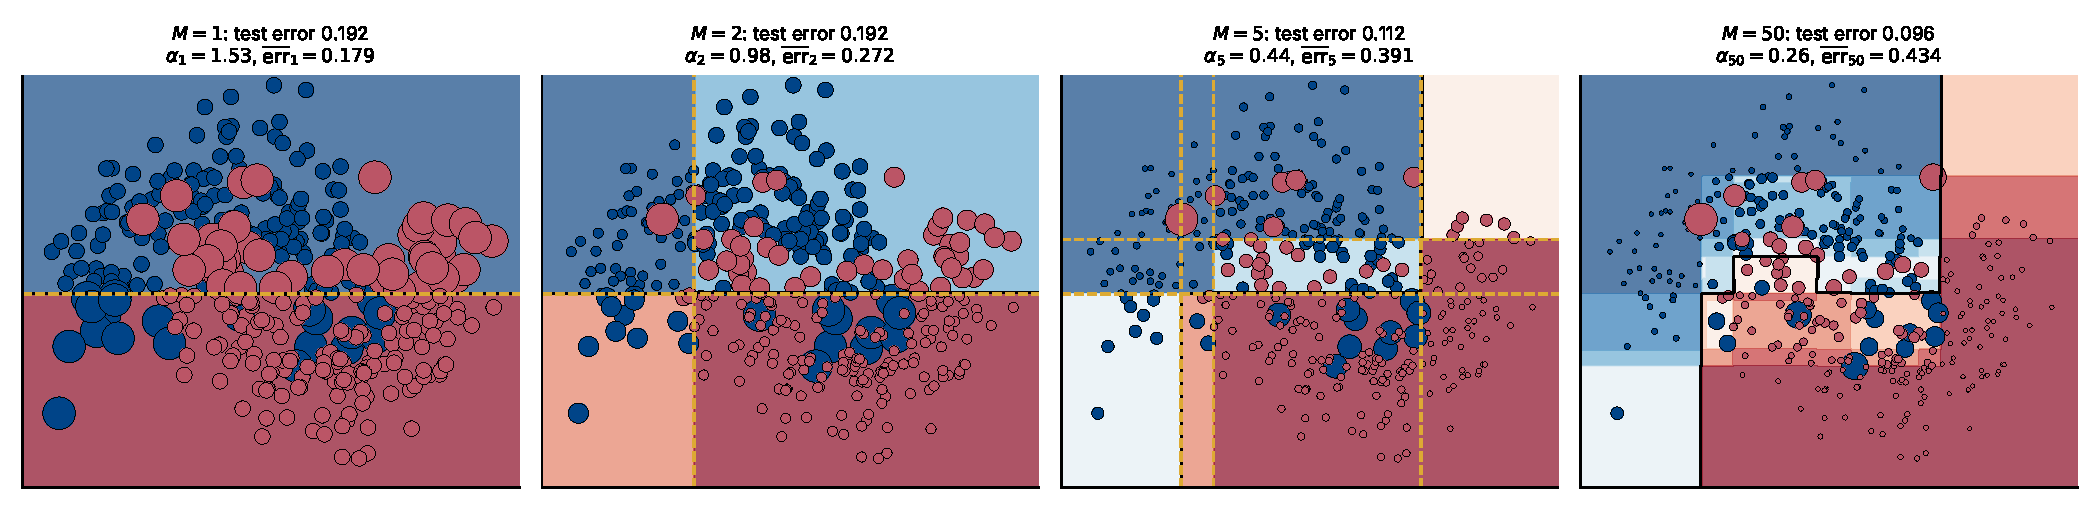
\includegraphics[width=0.99\textwidth]{week47_adaboost_rounds.pdf}\\
\small
Colour: the sign and size of $f_M=\sum_{m\leq M}\alpha_mG_m$; black line
$f_M=0$; the area of each training point is its weight $w_i$ after round
$M$; dashed lines are the stumps used so far.  The first stump is
horizontal ($x_2\leq0.16\Rightarrow$ class 0) and the tips of both
crescents, which lie on the wrong side of it, take the weight; the second
and third are vertical ($x_1\leq-0.39$, $x_1\leq1.53$) and cut those tips
off; by $M=5$ the weights sit on the overlap region and the boundary is a
staircase; by $M=50$ it is the sum of fifty thresholds -- jagged, but
tracking the crescents.
\end{frame}

\begin{frame}{Error, exponential loss and margins against the number of rounds}
\centering
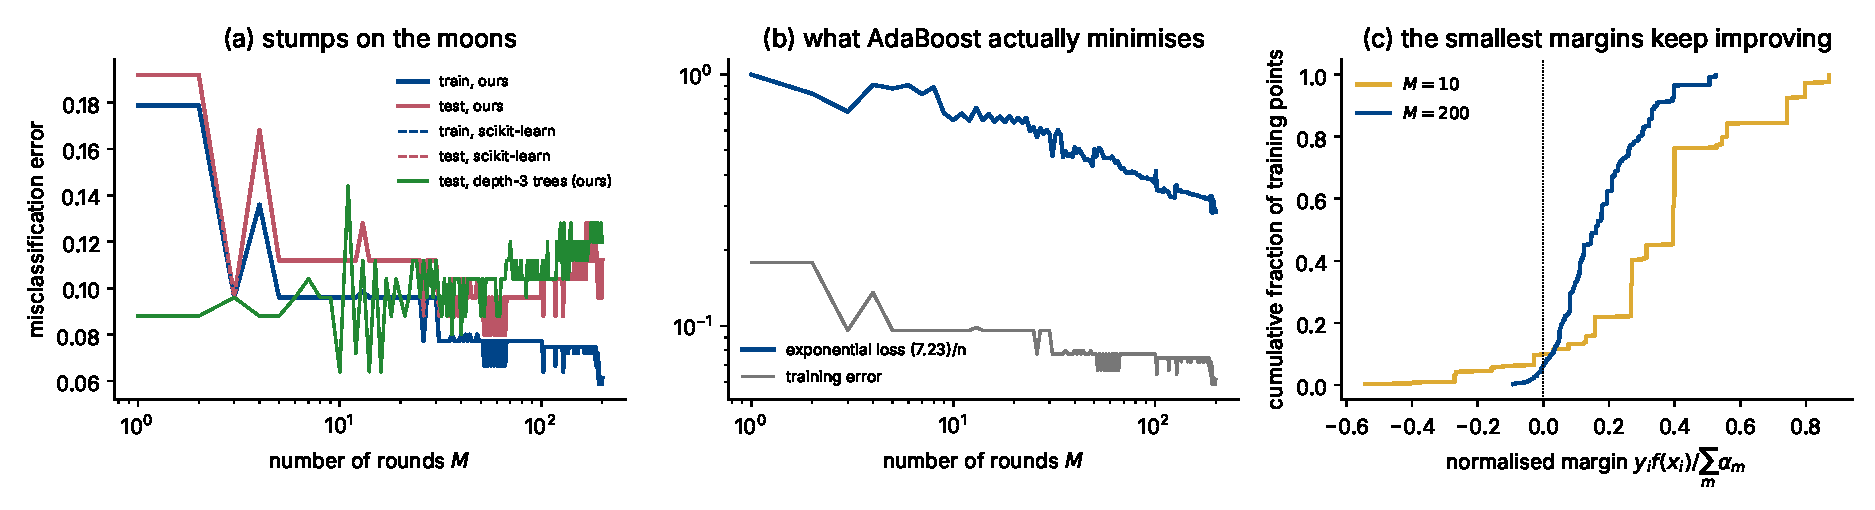
\includegraphics[width=0.99\textwidth]{week47_adaboost_error.pdf}\\
\small
\textbf{(a)} ours (solid) and \texttt{scikit-learn} (dashed) lie on top of
each other; green: depth-3 trees.  \textbf{(b)} the quantity AdaBoost
actually minimizes, $\frac1n\sum_ie^{-y_if_M(\bm{x}_i)}$, falls
monotonically while the 0--1 training error moves in steps and plateaus:
the algorithm is a coordinate descent on (7.23), not on the error.
\textbf{(c)} the cumulative distribution of the normalized margins
$y_if(\bm{x}_i)/\sum_m\alpha_m$: from $M=10$ to $M=200$ the \emph{smallest}
margin rises from $-0.54$ to $-0.09$ and the fraction with negative margin
from $0.096$ to $0.061$, while the median decreases -- the ensemble spends
its later rounds on the hardest points, and the margin of the easy ones is
traded away.
\end{frame}

\begin{insight}[is AdaBoost immune to overfitting?]
\question{The depth-3 ensemble reaches zero training error at $M=50$, and
its test error then rises from $0.088$ to $0.120$ by $M=200$.  The folklore
says boosting ``does not overfit''.  Who is right?}
\answer{The data.  The folklore comes from clean benchmarks where the test
error keeps improving long after the training error is zero, and the margin
argument explains why it \emph{can}.  But the moons have label noise (about
$8\%$ of the points are on the wrong side of the Bayes boundary), and the
exponential loss gives a point with margin $-3$ twenty times the weight of a
point with margin $0$; the later trees are fitted almost entirely to those
noisy points and carve islands around them -- exactly the single-tree
pathology we averaged away last week.  Three remedies, all in use: a
\textbf{smaller step} (\texttt{learning\_rate}$<1$, shrinkage), a
\textbf{robust loss} (logistic, Huber -- gradient boosting, next part), and
\textbf{choosing $M$ by validation} (early stopping) instead of ``as large
as you can afford'', which was the right answer for bagging and is the wrong
one here.}
\end{insight}

%% =====================================================================
\section{Steepest descent in function space (Section 7.13)}
%% =====================================================================

\begin{frame}{From AdaBoost to any loss: the gradient with respect to the predictions}
\begin{columns}[T]
\begin{column}{0.54\textwidth}
\footnotesize
Stagewise fitting with an arbitrary differentiable loss $L$ has no closed
form.  Friedman's idea (2001): treat the $n$ predicted values
$\bm{f}=(f(\bm{x}_1),\dots,f(\bm{x}_n))^T$ as the parameters and do
\textbf{gradient descent on the training loss}
\[
\mathcal{L}(\bm{f})=\sum_{i=1}^n L\big(y_i,f(\bm{x}_i)\big).
\]
The gradient at the current model $f_{m-1}$ has components
\[
g_{im}=\left[\frac{\partial L(y_i,f(\bm{x}_i))}{\partial f(\bm{x}_i)}\right]_{f=f_{m-1}},\tag{7.30}
\]
and steepest descent with an exact line search is
\[
\rho_m=\arg\min_\rho\mathcal{L}(\bm{f}_{m-1}-\rho\,\bm{g}_m),\qquad
\bm{f}_m=\bm{f}_{m-1}-\rho_m\bm{g}_m .
\]
Each step adds a ``function'' $-\rho_m\bm{g}_m$: this \emph{is} an additive
model, Eq.\ (7.19), with the negative gradient as the $m$-th basis function.
\end{column}
\begin{column}{0.46\textwidth}
\footnotesize
\begin{block}{The squared error worked out}
$L=\frac12(y-f)^2$ gives $g_{im}=-(y_i-f_{m-1}(\bm{x}_i))$: the negative
gradient \textbf{is the residual}.  Start from $f_0=0$: $\bm{g}_1=-\bm{y}$.
Line search:
\[
\rho_1=\arg\min_\rho\tfrac12\|\bm{y}-\rho\bm{y}\|^2
\;\Rightarrow\;\rho_1=1 ,\qquad \bm{f}_1=\bm{y}.
\]
(With $L=(y-f)^2$ the gradient is $-2(\bm{y}-\bm{f})$ and $\rho_1=\frac12$;
same $\bm{f}_1$.)  \textbf{One step fits every training point exactly}, the
training loss is zero, and $\rho_2=0$ -- our code prints
\texttt{rho\_1 = 0.5000, training MSE 0.00e+00, rho\_2 = 0.0000}.
\end{block}
\begin{block}{And that is the problem}
$\bm{f}_1$ is a list of $n$ numbers at $n$ points.  It says \emph{nothing}
about any other $\bm{x}$ -- there is no function to evaluate on the test set
-- and it has interpolated the noise.  Steepest descent in function space,
taken literally, is the perfect overfitter with zero generalization.
\end{block}
\end{column}
\end{columns}
\end{frame}

\begin{frame}{The repair: take the step along a tree instead of along the gradient}
\begin{columns}[T]
\begin{column}{0.5\textwidth}
\footnotesize
We want a step that (i) points roughly along $-\bm{g}_m$ at the training
points and (ii) is a \emph{function} defined everywhere, from a class with
limited capacity.  So \textbf{fit a regression tree $T_m$ to the negative
gradient}:
\[
T_m=\arg\min_T\sum_{i=1}^n\big(-g_{im}-T(\bm{x}_i)\big)^2 ,
\]
the squared-error projection of the steepest-descent direction onto the
set of trees with $J$ leaves.  Then step along $T_m$:
\[
f_m(\bm{x})=f_{m-1}(\bm{x})+\nu\,\rho_m T_m(\bm{x}),
\]
\[
\rho_m=\arg\min_\rho\sum_iL\big(y_i,f_{m-1}(\bm{x}_i)+\rho T_m(\bm{x}_i)\big).
\]
With a tree the line search is done \textbf{leaf by leaf}: the tree fixes
the regions $R_{jm}$, and the value in each region is
\[
\gamma_{jm}=\arg\min_\gamma\sum_{\bm{x}_i\in R_{jm}}L\big(y_i,f_{m-1}(\bm{x}_i)+\gamma\big),
\]
$J$ one-dimensional problems instead of one.
\end{column}
\begin{column}{0.5\textwidth}
\begin{block}{Gradient boosting: the algorithm}
\footnotesize
\begin{enumerate}
  \item $f_0(\bm{x})=\arg\min_\gamma\sum_iL(y_i,\gamma)$ -- the best
    constant ($\bar y$ for the squared error, the log-odds for the logistic
    loss).
  \item For $m=1,\dots,M$:
  \begin{enumerate}
    \item[(a)] pseudo-residuals $u_{im}=-g_{im}$, Eq.\ (7.30);
    \item[(b)] fit a regression tree to $\{(\bm{x}_i,u_{im})\}$, giving
      regions $R_{jm}$, $j=1,\dots,J_m$;
    \item[(c)] leaf values $\gamma_{jm}$ by the one-dimensional line search
      above;
    \item[(d)] $f_m(\bm{x})=f_{m-1}(\bm{x})+\nu\sum_j\gamma_{jm}I(\bm{x}\in R_{jm})$.
  \end{enumerate}
  \item Output $f_M$.
\end{enumerate}
\end{block}
\footnotesize
For the squared error this is literally \textbf{``fit a tree to the
residuals and add it''}, Eq.\ (7.31): the leaf values are mean residuals,
so (b) and (c) coincide.  $\nu\in(0,1]$ is the \textbf{shrinkage}.
\end{column}
\end{columns}
\end{frame}

\begin{frame}{Pseudo-residuals for the losses you will use}
\footnotesize
\begin{center}
\scriptsize
\begin{tabular}{@{}llll@{}}
\toprule
task & loss $L(y,f)$ & $u=-\partial L/\partial f$ & leaf value $\gamma_j$\\
\midrule
regression & $\frac12(y-f)^2$ & $y-f$ \quad (7.31) & mean of $u$ in the leaf\\
regression, robust & $|y-f|$ & $\sgn(y-f)$ & median of $y-f$ in the leaf\\
regression, Huber & quadratic, linear beyond $\pm\delta$ & $y-f$ clipped at $\pm\delta$ & robust location\\
two classes, $y\in\{0,1\}$ & binomial deviance, $p=\sigma(f)$ & $y-p$ \quad (7.32) & $\sum u/\sum p(1-p)$ (Newton)\\
$K$ classes & multinomial deviance, softmax & $y_k-p_k$, one tree per class & Newton per class\\
\bottomrule
\end{tabular}
\normalsize
\end{center}
\begin{columns}[T]
\begin{column}{0.5\textwidth}
\begin{block}{The logistic case, Eq.\ (7.32)}
With $p=\sigma(f)=1/(1+e^{-f})$ and $\partial p/\partial f=p(1-p)$,
\[
-\frac{\partial L}{\partial f}=-\Big[-\frac{y}{p}+\frac{1-y}{1-p}\Big]p(1-p)=y-p ,
\]
the same ``observed minus predicted'' residual as in logistic regression
and in a network's cross-entropy output layer.  Gradient boosting fits
trees to $y-p$ and adds them to the \emph{log-odds}.
\end{block}
\end{column}
\begin{column}{0.5\textwidth}
\begin{block}{The leaf value is a Newton step}
For the logistic loss the line search in a leaf has no closed form; one
Newton step from $\gamma=0$ gives
\[
\gamma_j=\frac{\sum_{i\in R_j}(y_i-p_i)}{\sum_{i\in R_j}p_i(1-p_i)}
=-\frac{\sum_i g_i}{\sum_i h_i},
\]
first over second derivatives.  Keep it: XGBoost is built on it, with a
$+\lambda$ in the denominator.
\end{block}
\end{column}
\end{columns}
\end{frame}

%% =====================================================================
\section{Gradient boosting with scikit-learn}
%% =====================================================================

\begin{frame}[fragile]{Code 3: our own gradient-boosting regressor, and the library}
\begin{columns}[T]
\begin{column}{0.5\textwidth}
\footnotesize
Section 7.13, squared error, last week's regression tree on the residuals:
\begin{lstlisting}[basicstyle=\ttfamily\tiny]
class GradientBoostingRegressor:
    def __init__(self, n_estimators=100, learning_rate=0.1, max_depth=3):
        self.n_estimators, self.lr, self.max_depth = n_estimators, learning_rate, max_depth

    def fit(self, X, y):
        self.f0_ = y.mean()                        # the best constant
        f = np.full(len(y), self.f0_)
        self.trees_ = []
        for _ in range(self.n_estimators):
            residual = y - f                       # negative gradient, Eq. (7.31)
            tree = DecisionTree("regression", max_depth=self.max_depth).fit(X, residual)
            f = f + self.lr * tree.predict(X)      # shrunken step
            self.trees_.append(tree)
        return self

    def predict(self, X, M=None):
        f = np.full(X.shape[0], self.f0_)
        for tree in self.trees_[:M]:
            f = f + self.lr * tree.predict(X)
        return f
\end{lstlisting}
Depth 2, $\nu=0.1$, $M=100$: test MSE \textbf{ours $0.0128$},
\textbf{\texttt{scikit-learn} $0.0113$}, noise $0.0100$.  The library's
trees use Friedman's improved MSE split criterion and break ties
differently; the algorithm is the same.
\end{column}
\begin{column}{0.5\textwidth}
\footnotesize
The data of the DocOnce notes: $n=100$ points, $x\in[-3,3]$,
\[
y=e^{-x^2}+\tfrac32e^{-(x-2)^2}+\epsilon,\quad\epsilon\sim N(0,0.1^2),
\]
80 for training, 20 for testing.
\begin{lstlisting}[basicstyle=\ttfamily\tiny]
from sklearn.ensemble import GradientBoostingRegressor
gb = GradientBoostingRegressor(max_depth=2, learning_rate=0.1,
         n_estimators=300, random_state=2026).fit(Xtr, ytr)
fits = list(gb.staged_predict(xgrid))      # f_1, f_2, ..., f_300 on a grid
test_mse = [np.mean((p - yte)**2) for p in gb.staged_predict(Xte)]
\end{lstlisting}
\begin{block}{Arguments worth knowing}
\begin{itemize}
  \item \texttt{loss}: \texttt{squared\_error}, \texttt{absolute\_error},
    \texttt{huber}, \texttt{quantile} -- the table two slides back;
  \item \texttt{subsample}$<1$: stochastic gradient boosting;
  \item \texttt{n\_iter\_no\_change}, \texttt{validation\_fraction}: early stopping;
  \item \texttt{max\_depth} / \texttt{max\_leaf\_nodes}: the interaction order.
\end{itemize}
\end{block}
\end{column}
\end{columns}
\end{frame}


\begin{frame}{Steepest descent, staged fits, residuals and the $\nu$--$M$ trade-off}
\centering
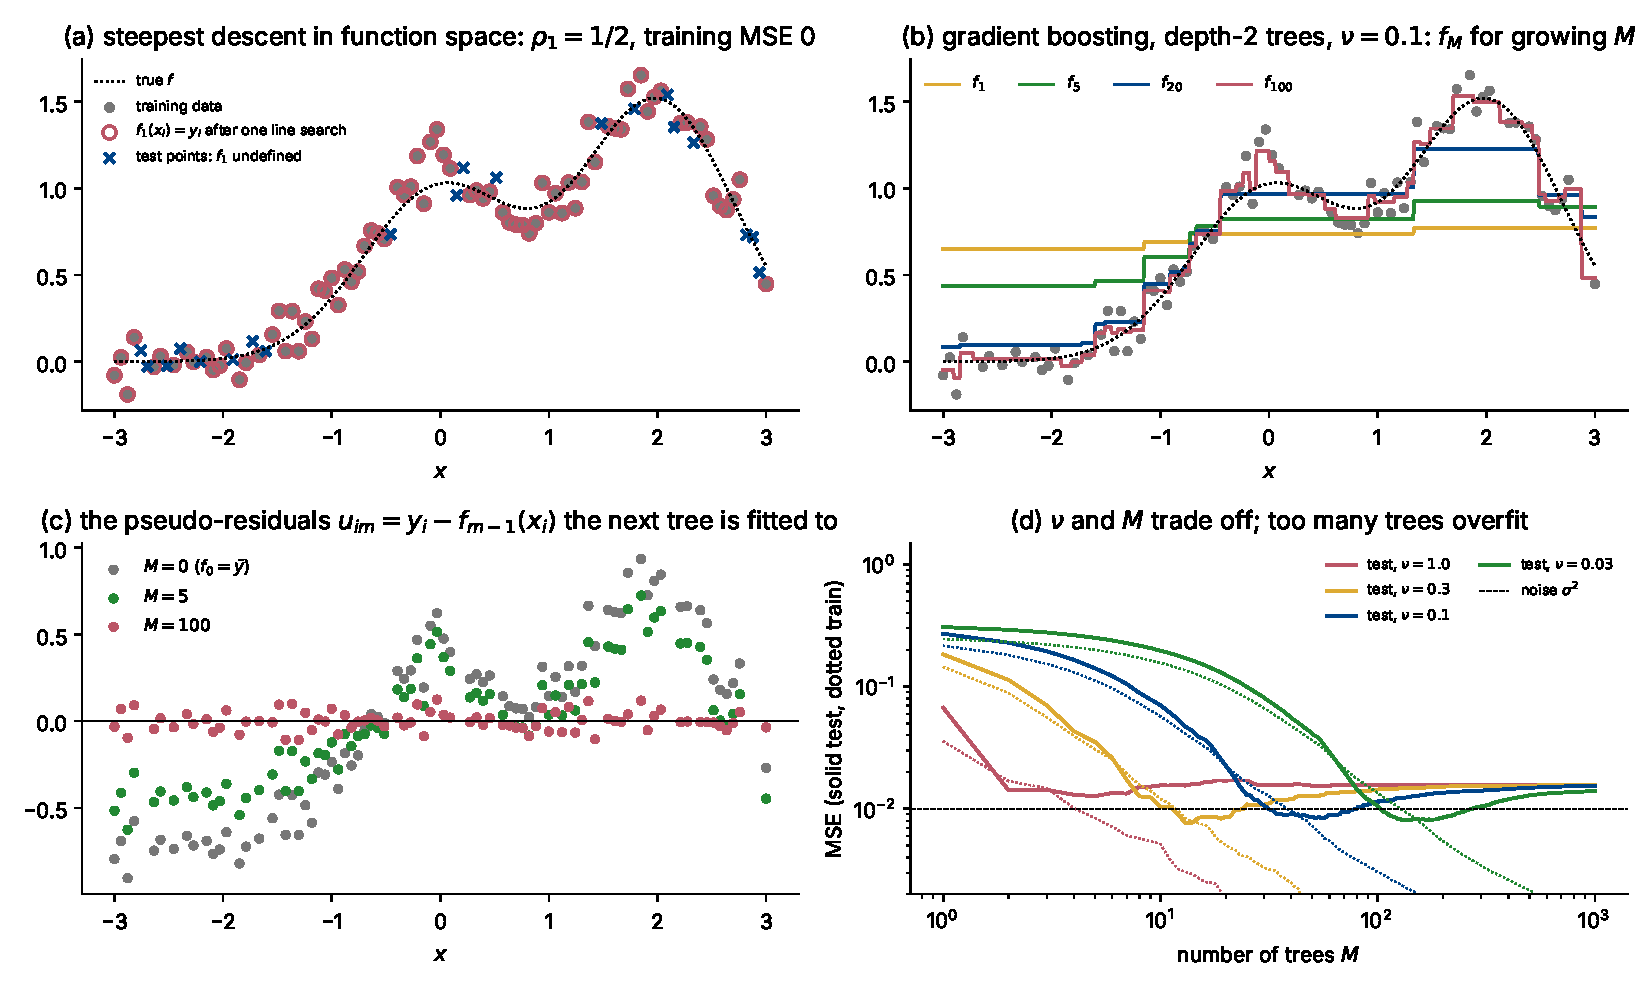
\includegraphics[height=0.72\textheight]{week47_gb_regression.pdf}\\
\scriptsize
\textbf{(a)} literal steepest descent: after one line search $f_1(x_i)=y_i$
at every training point (red circles), and $f_1$ does not exist at the test
points (blue crosses).  \textbf{(b)} gradient boosting with depth-2 trees:
$f_1$ is a two-split staircase, $f_{100}$ follows the two bumps.
\textbf{(c)} the pseudo-residuals $u_{im}=y_i-f_{m-1}(x_i)$ the next tree
sees: structure at $M=0$, structure at $M=5$, noise at $M=100$.
\textbf{(d)} test MSE against $M$ for four learning rates.
\end{frame}

\begin{frame}{Shrinkage: $\nu$ and $M$ are not independent knobs}
\begin{columns}[T]
\begin{column}{0.5\textwidth}
\footnotesize
Panel (d) in numbers (depth 2, up to 1000 trees):
\begin{center}
\scriptsize
\begin{tabular}{@{}rrrr@{}}
\toprule
$\nu$ & best $M$ & best test & at $M{=}1000$\\
\midrule
1.00 & 5   & 0.0127 & 0.0155\\
0.30 & 13  & 0.0076 & 0.0155\\
0.10 & 56  & 0.0084 & 0.0154\\
0.03 & 137 & 0.0080 & 0.0140\\
\bottomrule
\end{tabular}
\end{center}
\begin{itemize}
  \item Smaller $\nu$ needs proportionally more trees: $\nu M\approx$
    constant at the optimum ($5$, $3.9$, $5.6$, $4.1$).
  \item Smaller $\nu$ reaches a \textbf{lower minimum} and degrades more
    slowly past it; $\nu=1$ overfits after five trees.
  \item Every curve eventually rises: unlike bagging, \textbf{more trees is
    not free}.  The training MSE (dotted) goes to zero for $\nu=1$ within a
    hundred trees -- the ensemble has interpolated the noise.
\end{itemize}
\end{column}
\begin{column}{0.5\textwidth}
\begin{block}{Why small steps generalize better}
\footnotesize
Stagewise fitting with a small $\nu$ traces a \emph{regularization path}:
after $M$ steps the model has moved a distance of order $\nu M$ from the
constant, in small increments that each take the direction of the current
residual.  Early stopping on this path behaves like the $\ell_1$ /
$\ell_2$ penalties of week 36 -- for a linear basis one can show the
stagewise path with $\nu\to0$ coincides with the lasso path (Efron et al.
2004).  Large steps commit early to the first residual's shape, noise
included; small steps keep correcting.  The price is computation, which is
why $\nu\in[0.01,0.1]$ with $M$ chosen by validation is the universal
recipe.
\end{block}
\begin{block}{The other knobs}
\footnotesize
\textbf{Depth} $d$ (interaction order; $d=2$--$6$ is typical, stumps for
additive problems), \textbf{subsample} $<1$ (a random half of the data per
tree -- variance reduction \emph{inside} boosting, Friedman 2002),
\textbf{min samples per leaf}, and the \textbf{loss}.
\end{block}
\end{column}
\end{columns}
\end{frame}

\begin{insight}[where did the bias go?]
\question{Each depth-2 tree is a piecewise constant with at most four
pieces -- a terrible approximation to two smooth bumps.  Yet $f_{100}$ in
panel (b) follows them closely.  Where did the bias of the weak learner go,
and why does the same not happen when we \emph{bag} depth-2 trees?}
\answer{Into the sum.  Every tree is fitted to the \emph{residual} of the
previous ones, so its four pieces are placed where the current error is
largest; a hundred trees give up to a few hundred distinct cutpoints,
arranged adaptively -- a piecewise constant with hundreds of pieces whose
positions were chosen by the data.  That is a rich class; the bias is small.
Bagged depth-2 trees are all fitted to the \emph{same} target, so their
cutpoints cluster around the same few positions (the biggest drops of the
function) and the average is a slightly smoothed four-piece staircase: the
same bias as one tree, Eq.\ (7.16) in action.  Boosting reduces bias
sequentially; bagging reduces variance in parallel.  (Boosting also reduces
variance when $\nu$ is small and \texttt{subsample}$<1$ -- but that is a
bonus, not the mechanism.)}
\end{insight}

\begin{frame}{Classification: the logistic loss on the moons, against AdaBoost}
\centering
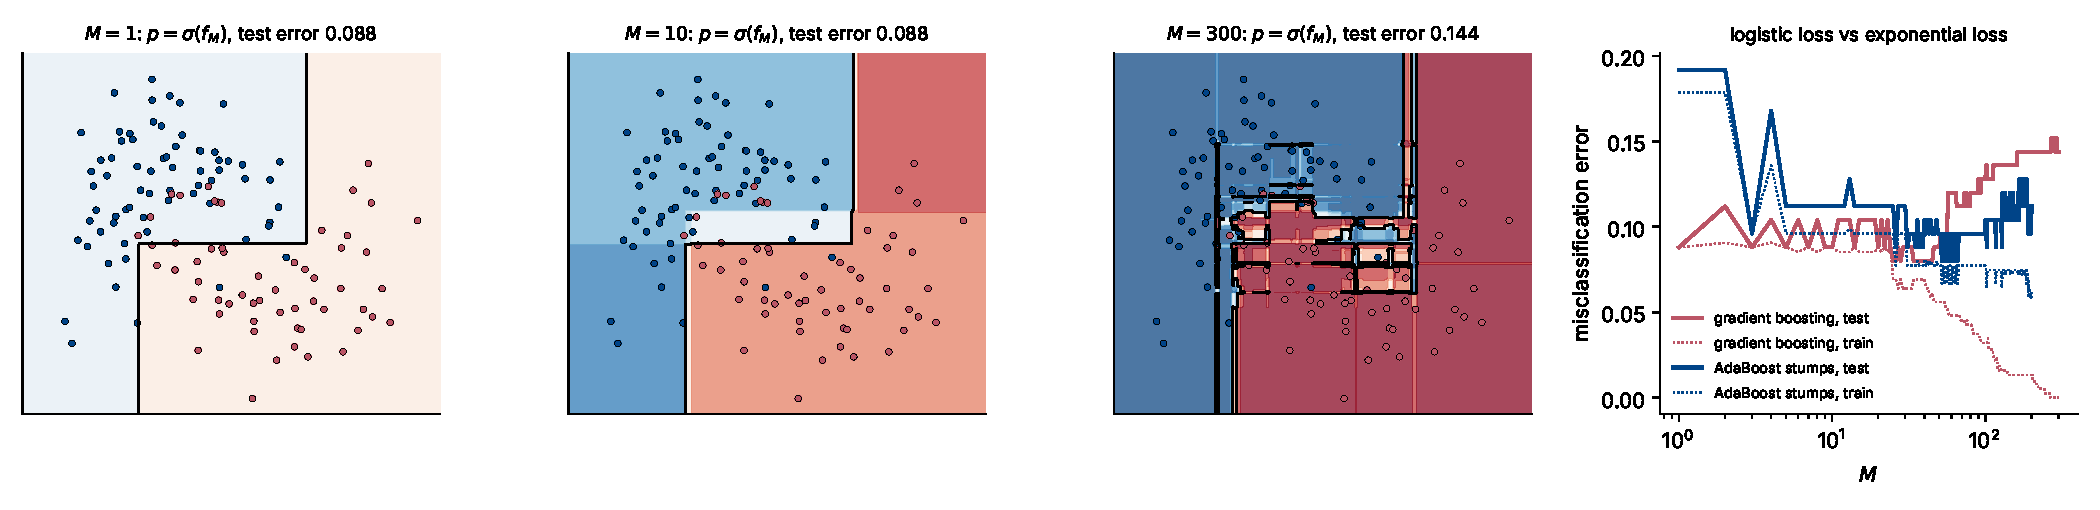
\includegraphics[width=0.99\textwidth]{week47_gb_moons.pdf}\\
\small
\texttt{GradientBoostingClassifier(max\_depth=2, learning\_rate=0.1)}: the
colour is $p=\sigma(f_M)$, a \emph{probability}, which AdaBoost's
$\sgn f$ never gave us.  Test error $0.088$ at $M=1$ and $M=10$, best
$0.080$ at $M=25$ -- the Bayes error -- then $0.128$ at $M=100$ and $0.144$
at $M=300$ as the islands appear.  Right: against AdaBoost stumps (blue).
Both overfit eventually; gradient boosting with the logistic loss gets
\emph{lower} first, with depth-2 trees that can represent the crescents, and
the cure is the same: stop early.  Note the training error of gradient
boosting reaching zero while the test error climbs.
\end{frame}

%% =====================================================================
\section{XGBoost (Section 7.14)}
%% =====================================================================

\begin{frame}{XGBoost (Chen and Guestrin 2016): second-order boosting with regularized trees}
\begin{columns}[T]
\begin{column}{0.56\textwidth}
\footnotesize
Gradient boosting uses the first derivative to choose the direction and a
line search for the step.  XGBoost expands the loss at stage $m$ to
\textbf{second order} in the new tree $T(\bm{x})$ (Newton instead of
steepest descent), and adds an explicit \textbf{penalty on the tree}:
\[
\mathcal{L}^{(m)}\approx\sum_{i}\Big[g_iT(\bm{x}_i)+\tfrac12h_iT(\bm{x}_i)^2\Big]+\Omega(T),\tag{7.33}
\]
\[
g_i=\frac{\partial L(y_i,f)}{\partial f}\Big|_{f_{m-1}(\bm{x}_i)},\qquad
h_i=\frac{\partial^2L(y_i,f)}{\partial f^2}\Big|_{f_{m-1}(\bm{x}_i)},
\]
\[
\Omega(T)=\gamma\,J+\tfrac12\lambda\sum_{j=1}^Jw_j^2,\tag{7.34}
\]
for a tree with $J$ leaves and leaf values $w_j$: $\gamma$ charges for every
leaf, $\lambda$ is a ridge penalty on the leaf values; the constant
$L(y_i,f_{m-1})$ was dropped.

\end{column}
\begin{column}{0.42\textwidth}
\begin{block}{$g_i$ and $h_i$ for the usual losses}
\footnotesize
\setlength{\tabcolsep}{4pt}%
\begin{tabular}{@{}lll@{}}
\toprule
loss & $g_i$ & $h_i$\\
\midrule
$\frac12(y-f)^2$ & $f_{m-1}(\bm{x}_i)-y_i$ & $1$\\
logistic, $p=\sigma(f)$ & $p_i-y_i$ & $p_i(1-p_i)$\\
Poisson, $\mu=e^{f}$ & $\mu_i-y_i$ & $\mu_i$\\
\bottomrule
\end{tabular}
\medskip

The same $g$ and $h$ as in the Newton leaf step of the previous part.  Any
loss with two derivatives works -- including one you write yourself
(Section 7.15).
\end{block}
\begin{block}{Why second order}
\footnotesize
Newton's method has the step built in, $-g/h$, and a quadratic model is
what makes leaf values and split score come out in closed form.
\end{block}
\end{column}
\end{columns}
\end{frame}

\begin{frame}{The leaf values and the score of a tree, in closed form}
\begin{columns}[T]
\begin{column}{0.54\textwidth}
\footnotesize
A tree is $T(\bm{x})=w_{q(\bm{x})}$ with $q$ the leaf index.  Group the sum
by leaf, $I_j=\{i:q(\bm{x}_i)=j\}$:
\[
\mathcal{L}^{(m)}\approx\sum_{j=1}^J\Big[G_jw_j+\tfrac12(H_j+\lambda)w_j^2\Big]+\gamma J,\tag{7.35}
\]
\[
G_j=\sum_{i\in I_j}g_i,\qquad H_j=\sum_{i\in I_j}h_i .
\]
Each leaf is a separate quadratic in $w_j$; minimizing,
\[
w_j^*=-\frac{G_j}{H_j+\lambda},\quad
\mathcal{L}^{(m)*}=-\frac12\sum_{j=1}^J\frac{G_j^2}{H_j+\lambda}+\gamma J .\tag{7.36}
\]
\begin{block}{Two things we gained}
\begin{itemize}
  \item the \textbf{leaf values in closed form} for \emph{any} twice
    differentiable loss -- no line search, no per-loss code;
  \item a \textbf{score for a tree structure} that does not depend on the
    leaf values, so it can be used to \emph{grow} the tree.
\end{itemize}
\end{block}
\end{column}
\begin{column}{0.46\textwidth}
\begin{block}{Reading Eq.\ (7.36)}
\footnotesize
\begin{itemize}
  \item $w_j^*=-G_j/(H_j+\lambda)$ is a \textbf{Newton step} per leaf, damped
    by $\lambda$: the sum of the gradients over the sum of the curvatures.
  \item The score $-\frac12\sum_jG_j^2/(H_j+\lambda)+\gamma J$ is the best
    the tree structure can do; the smaller, the better.  It plays the role
    of the impurity in CART.
  \item For the squared error ($h_i=1$, $\lambda=0$) the leaf value is the
    mean residual $-G_j/n_j$: gradient boosting as before.
  \item Every quantity is a \textbf{sum over the points in a leaf} -- what
    makes histogram binning and parallel split finding possible.
\end{itemize}
\end{block}
\end{column}
\end{columns}
\end{frame}

\begin{frame}{The gain of a split}
\begin{columns}[T]
\begin{column}{0.56\textwidth}
\footnotesize
A split of leaf $I$ into $I_L\cup I_R$ changes the score (7.36) by
\[
\mathrm{Gain}=\tfrac12\Big[\tfrac{G_L^2}{H_L+\lambda}+\tfrac{G_R^2}{H_R+\lambda}
-\tfrac{(G_L+G_R)^2}{H_L+H_R+\lambda}\Big]-\gamma .\tag{7.37}
\]
Grow the tree greedily on this gain, as CART grows on the impurity
decrease; a split with $\mathrm{Gain}<0$ is not made -- $\gamma$ is a
\textbf{built-in pruning threshold}, and $\lambda$ \textbf{shrinks} leaves
with little curvature $H_j$ toward zero.
\begin{block}{Growing one tree on the gain}
\begin{enumerate}
  \item Compute $g_i$, $h_i$ once per round (they depend on $f_{m-1}$ only).
  \item For every feature and candidate threshold (histogram bin edges),
    accumulate $G_L,H_L$ in one sweep, $G_R=G-G_L$, $H_R=H-H_L$, evaluate
    (7.37).
  \item Take the best split if its gain is positive; recurse to
    \texttt{max\_depth}, with \texttt{min\_child\_weight} bounding $H_L,H_R$.
  \item Leaf values from (7.36) times $\nu$; add the tree, next round.
\end{enumerate}
\end{block}

\end{column}
\begin{column}{0.44\textwidth}
\begin{block}{A leaf by hand (logistic loss)}
\footnotesize
Three points in a leaf, labels $y=(1,0,1)$, current probabilities
$p=(0.6,0.6,0.6)$:
\[
g=p-y=(-0.4,\,0.6,\,-0.4),\qquad G=-0.20,
\]
\[
h=p(1-p)=(0.24,\,0.24,\,0.24),\qquad H=0.72 .
\]
Unregularized Newton step: $w^*=-G/H=0.278$ (push the log-odds up: two
of three are positive, $p=0.6$ was too low).  With $\lambda=1$:
$w^*=-G/(H+\lambda)=0.20/1.72=\mathbf{0.116}$, less than half -- because
$H=0.72<\lambda$, a leaf of three points has little curvature to back its
estimate.  Score of the leaf: $-\frac12G^2/(H+\lambda)=-0.0116$.  Compare
$\lambda$ with $H_j$, not with $n_j$: that is the meaning of
\texttt{min\_child\_weight} (a lower bound on $H_j$) in the library.
\end{block}

\end{column}
\end{columns}
\end{frame}

\begin{frame}{Sanity check: with the squared error XGBoost is CART on the residuals}
\begin{columns}[T]
\begin{column}{0.56\textwidth}
\footnotesize
\textbf{Check}: squared error, $h_i=1$, $\lambda=\gamma=0$.  Then
$G_j=-\sum_{I_j}r_i$ with $r_i$ the residual, $H_j=n_j$, and
\[
\mathrm{Gain}=\frac12\Big[n_L\bar r_L^2+n_R\bar r_R^2-n\,\bar r^2\Big],\tag{7.38}
\]
which is exactly the decrease in the residual sum of squares of CART's
regression split, Eqs.\ (7.11)--(7.12) of last week (expand
$\sum(r_i-\bar r)^2=\sum r_i^2-n\bar r^2$).  So XGBoost with the squared
loss and no regularization \emph{is} gradient boosting with CART trees and
the mean residual in each leaf; everything else is the second-order
treatment of other losses and the two penalties.
\end{column}
\begin{column}{0.44\textwidth}
\begin{block}{Multiply by $\nu$}
\footnotesize
The actual update is $f_m=f_{m-1}+\nu\,T_m$ with $\nu$ (\texttt{eta},
\texttt{learning\_rate}) typically $0.01$--$0.3$; the leaf weights of Eq.\
(7.36) are the full Newton step.
\end{block}
\begin{block}{What is new, then}
\footnotesize
\begin{itemize}
  \item the second-order treatment of \emph{other} losses -- the logistic
    leaf is $-G/(H+\lambda)$ with no line search;
  \item $\lambda$ shrinks the small leaves, $\gamma$ prunes while growing;
  \item the same gain drives the split search for every loss, so the tree
    code is written once.
\end{itemize}
\end{block}
\end{column}
\end{columns}
\end{frame}

\begin{insight}[what does $\lambda$ do to a leaf with a single point?]
\question{Squared error, one training point in a leaf with residual $r$.
What are $G$, $H$ and $w^*$ for $\lambda=0$, $1$, $10$?  What does the
answer say about the role of $\lambda$ in a deep tree versus a shallow
one, and what is the analogous quantity in ridge regression?}
\answer{$g=-r$, $h=1$, so $G=-r$, $H=1$ and $w^*=r/(1+\lambda)$: the full
residual for $\lambda=0$, half of it for $\lambda=1$, a tenth for
$\lambda=10$.  A leaf with $n_j$ points has $H_j=n_j$ and
$w^*=\bar r_j\,n_j/(n_j+\lambda)$: the shrinkage factor $n_j/(n_j+\lambda)$
is negligible for large leaves and strong for small ones -- $\lambda$ acts
almost entirely on the \textbf{small leaves of deep trees}, the ones that fit
single noisy points.  It is ridge regression's $\beta_j\to\beta_j\,
d_j^2/(d_j^2+\lambda)$ of week 36 with the singular value replaced by the
leaf's curvature.  On the cancer data below, raising $\lambda$ from $0$ to
$10$ \emph{increased} the mean number of leaves per tree from 3 to 5: with
shrunken leaves the probabilities stay away from $0$ and $1$, the $h_i$ stay
large, and more splits clear the \texttt{min\_child\_weight} and $\gamma$
thresholds.  The knobs interact.}
\end{insight}

\begin{frame}{What else is in the box}
\footnotesize
\begin{columns}[T]
\begin{column}{0.5\textwidth}
\begin{block}{Statistics}
\begin{itemize}
  \item \textbf{Shrinkage} $\nu$ and \textbf{column subsampling} per tree
    or per split (\texttt{colsample\_bytree}, \texttt{\_bylevel}) -- the
    random-forest trick inside boosting -- and \textbf{row subsampling}
    (\texttt{subsample}).
  \item \textbf{Early stopping} on a validation set
    (\texttt{early\_stopping\_rounds}): choose $M$ by the held-out loss.
  \item \textbf{Any loss} with a gradient and a Hessian: regression,
    logistic, multinomial, Poisson, Cox survival, ranking -- or your own
    Python function returning $(g,h)$; Section 7.15 derives $g$ and $h$ by
    automatic differentiation.
  \item \textbf{Missing values}: each split learns a default direction for
    them (sparsity-aware split finding).
\end{itemize}
\end{block}
\end{column}
\begin{column}{0.5\textwidth}
\begin{block}{Engineering (where the ``X'' comes from)}
\begin{itemize}
  \item \textbf{Histogram split finding}: features are binned into
    $\leq256$ quantile buckets, so a split costs $O(\text{bins})$ instead of
    $O(n\log n)$; the \texttt{hist} method is the default.
  \item \textbf{Parallel} over features and over bins; GPU training;
    out-of-core blocks for data larger than memory.
  \item \texttt{scikit-learn}'s \texttt{HistGradientBoostingClassifier /
    Regressor} is the same design (binning, second-order leaves, $\ell_2$
    penalty, early stopping) and is 4--10 times faster than its older
    \texttt{GradientBoosting*} siblings; LightGBM and CatBoost are the other
    two libraries of the family.
\end{itemize}
\end{block}
\end{column}
\end{columns}
\medskip
On tabular data of moderate size, with heterogeneous features and
interactions, gradient-boosted trees have been the method to beat for a
decade; that is why Project 3's paths B and C both list them.
\end{frame}

\begin{frame}[fragile]{Code 4: XGBoost -- regression with early stopping, and the cancer data}
\begin{columns}[T]
\begin{column}{0.48\textwidth}
\begin{lstlisting}[basicstyle=\ttfamily\tiny]
import xgboost as xgb
reg = xgb.XGBRegressor(n_estimators=2000, learning_rate=0.05, max_depth=2,
                       reg_lambda=1.0, early_stopping_rounds=50, random_state=2026)
reg.fit(Xtr, ytr, eval_set=[(Xte, yte)], verbose=False)
reg.best_iteration                                    # 134
mse = np.mean((reg.predict(Xte) - yte)**2)
\end{lstlisting}
\footnotesize
Stops at $M=135$ (no improvement of the held-out loss for 50 rounds).  With
20 test points the test MSE is noisy -- XGBoost $0.0200$,
\texttt{scikit-learn} with the same $M$ $0.0090$ -- so we also measure the
error against the \emph{noise-free} function on a grid: XGBoost $0.0054$,
\texttt{scikit-learn} $0.0045$, both well below the noise variance
$0.0100$.  Same method, different defaults (\texttt{reg\_lambda=1},
\texttt{min\_child\_weight=1}, histogram bins).

\textbf{Honesty note}: stopping on the test set makes the test error
optimistic; in a project, hold out a \emph{third} set or cross-validate.
\end{column}
\begin{column}{0.52\textwidth}
\begin{lstlisting}[basicstyle=\ttfamily\tiny]
from sklearn.datasets import load_breast_cancer
from sklearn.ensemble import (RandomForestClassifier,
    GradientBoostingClassifier, HistGradientBoostingClassifier)
X, y = load_breast_cancer(return_X_y=True)
Xtr, Xte, ytr, yte = train_test_split(X, y, test_size=0.3, random_state=2026,
                                      stratify=y)
models = {
  "logistic":  make_pipeline(StandardScaler(), LogisticRegression(max_iter=5000)),
  "forest":    RandomForestClassifier(200, random_state=2026),
  "GB":        GradientBoostingClassifier(max_depth=3, learning_rate=0.1,
                                          n_estimators=200),
  "HistGB":    HistGradientBoostingClassifier(max_depth=3, learning_rate=0.1,
                                              max_iter=200),
  "XGBoost":   xgb.XGBClassifier(n_estimators=200, learning_rate=0.1, max_depth=3,
                                 reg_lambda=1.0, gamma=0.0, eval_metric="logloss")}
for name, m in models.items():
    m.fit(Xtr, ytr)
    p = m.predict_proba(Xte)[:, 1]
    print(name, m.score(Xte, yte), roc_auc_score(yte, p), log_loss(yte, p))

# logloss curves: fit with eval_set=[(Xtr, ytr), (Xte, yte)], read m.evals_result()
# importances:    m.get_booster().get_score(importance_type="gain")
\end{lstlisting}
\footnotesize
Five models, one loop, one \texttt{predict\_proba} interface -- the point
of \texttt{scikit-learn}'s API, which XGBoost implements.
\end{column}
\end{columns}
\end{frame}


\begin{frame}{The cancer data: five methods, three metrics}
\begin{columns}[T]
\begin{column}{0.56\textwidth}
\footnotesize
398 training, 171 test tumours, 30 features, seed 2026:
\begin{center}\scriptsize
\begin{tabular}{@{}lrrrr@{}}
\toprule
method & acc. & AUC & logloss & time\\
\midrule
logistic regression & \textbf{0.965} & \textbf{0.992} & \textbf{0.093} & 0.06 s\\
random forest, 200 trees        & 0.953 & 0.980 & 0.332 & 0.19 s\\
gradient boosting, $d=3$ & 0.953 & 0.988 & 0.238 & 0.40 s\\
hist gradient boosting & 0.959 & 0.985 & 0.229 & 0.11 s\\
XGBoost, $d=3$ & 0.947 & 0.986 & 0.138 & 0.05 s\\
\bottomrule
\end{tabular}
\end{center}
\begin{itemize}
  \item Accuracies differ by \textbf{at most three tumours} out of 171; the
    ranking by accuracy is not meaningful at this $n$.
  \item The \textbf{logloss} separates them: the forest's vote fractions are
    poorly calibrated ($0.33$), the boosted log-odds much better, XGBoost's
    $\lambda$ better still.  AUC says all five rank the tumours almost
    equally well.
  \item XGBoost is the fastest of the ensembles -- on 400 points.  The
    engineering shows at $n=4\cdot10^5$, not here.
\end{itemize}
\end{column}
\begin{column}{0.44\textwidth}
\footnotesize
\textbf{The $\lambda$--$\gamma$ scan} (XGBoost, 200 trees, depth 3):
\begin{center}\scriptsize
\begin{tabular}{@{}rrrrr@{}}
\toprule
$\lambda$ & $\gamma$ & acc. & logloss & leaves\\
\midrule
0  & 0 & 0.965 & 0.142 & 3\\
0  & 1 & 0.942 & 0.148 & 2\\
0  & 5 & 0.936 & 0.163 & 1\\
1  & 0 & 0.947 & 0.138 & 3\\
1  & 1 & 0.942 & 0.146 & 2\\
10 & 0 & 0.947 & 0.136 & 5\\
10 & 1 & 0.936 & 0.146 & 2\\
10 & 5 & 0.930 & 0.173 & 1\\
\bottomrule
\end{tabular}
\end{center}
$\gamma=5$ prunes every tree to a single leaf -- a constant per round, the
model degenerates to a slowly fitted intercept, and the error rises.
$\gamma=1$ leaves stumps.  $\lambda$ moves the logloss by a few
thousandths and the accuracy by one or two tumours.  On these data the
defaults ($\lambda=1$, $\gamma=0$) are as good as anything; the scan is how
you find out.
\end{column}
\end{columns}
\end{frame}

\begin{frame}{Logloss curves and importances}
\centering
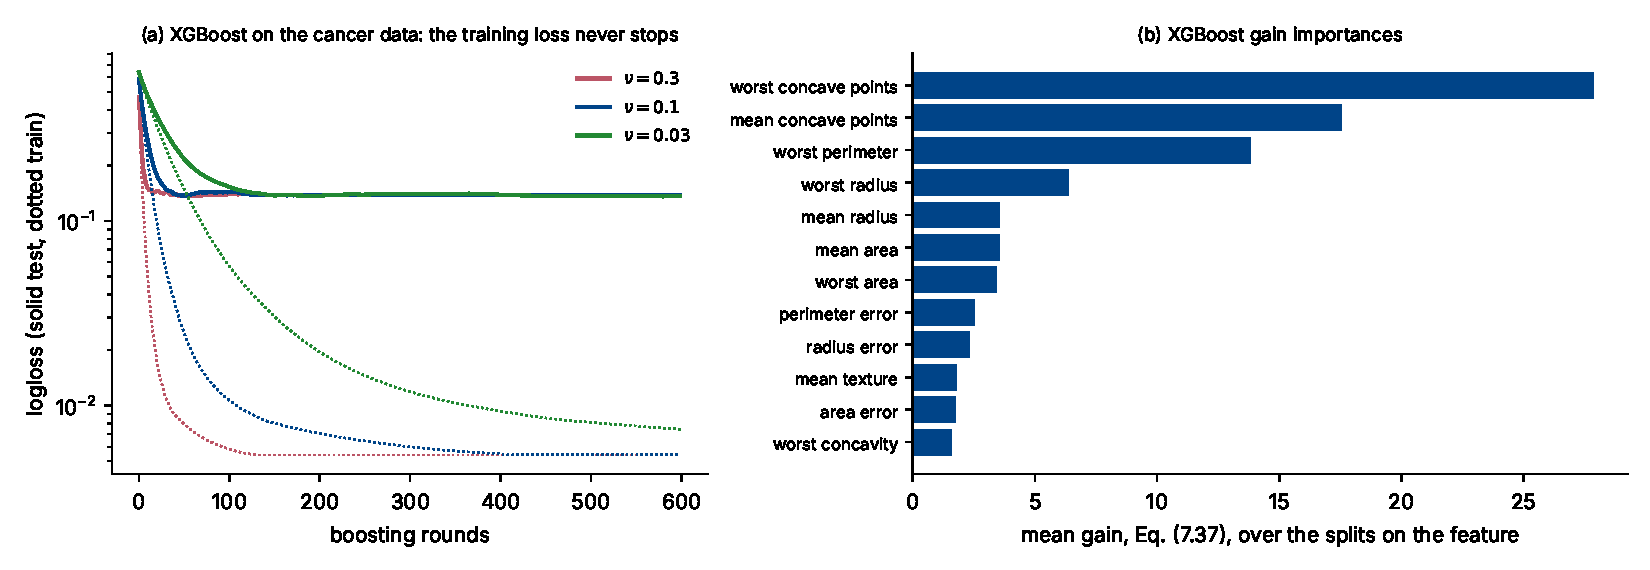
\includegraphics[width=0.95\textwidth]{week47_xgb_cancer.pdf}\\
\small
\textbf{(a)} test (solid) and training (dotted) logloss against the number
of rounds for three learning rates.  The training loss falls without end --
with $\nu=0.3$ to $10^{-3}$ -- while the test loss flattens at $0.13$--$0.15$
after 50--150 rounds and then creeps up: the picture to keep in mind
whenever \texttt{n\_estimators} is chosen by hand.  \textbf{(b)} gain
importances, Eq.\ (7.37) summed over the splits on each feature: the
concave-points, perimeter and radius features that the random forest
singled out last week, in a different order -- importances are
\emph{model} properties, not data properties.
\end{frame}

\begin{insight}[the simplest model won.  Why, and what should you do about it?]
\question{Logistic regression beats every tree ensemble on the cancer
data on all three metrics.  Why, and does that contradict the claim that
boosted trees are the method to beat on tabular data?}
\answer{Because the problem is \textbf{nearly linearly separable} in the
scaled features (the measurements are means and extremes of the same
geometric quantities, strongly correlated, and the classes differ by a
shift), the sample is small ($n=398$, $p=30$), and a linear model with 31
parameters has the right bias for exactly this situation -- the trees spend
their capacity reproducing a smooth oblique boundary with axis-aligned
steps.  No contradiction: the tabular-data claim is about data sets with
thousands to millions of rows, heterogeneous features, interactions and
missing values, where the linear model's bias dominates and the ensembles'
flexibility pays.  The lesson for Project 3 is procedural: \textbf{always
fit the simple baseline first} and report it next to the complicated
models; a method that does not beat logistic regression or OLS has not
earned its complexity -- and a method that does should be shown to do so on
a held-out set, not on the set you tuned it on.}
\end{insight}

%% =====================================================================
\section{Summary}
%% =====================================================================

\begin{frame}{Bagging against boosting, in one table}
\small
\begin{center}
\scriptsize
\begin{tabular}{@{}p{2.4cm}p{5.3cm}p{5.3cm}@{}}
\toprule
 & bagging / random forests (7.8--7.10) & boosting (7.11--7.15)\\
\midrule
members & deep trees: low bias, high variance & shallow trees: high bias, low variance\\
built & independently, in parallel & sequentially, each on the residual of the rest\\
combined & average or majority vote, equal weights & weighted sum, $\beta_m$ or $\alpha_m$ fitted\\
what it reduces & variance, down to the floor $\rho\sigma^2$, Eq.\ (7.16) & bias, stage by stage (and some variance)\\
the objective & none: a smoothing device & a loss, Eq.\ (7.20): exponential, logistic, squared, \dots\\
number of trees $B$, $M$ & as many as you can afford; never hurts & a tuning parameter; too many overfits\\
the main knobs & $m$ (features per split), tree depth & $\nu$, $M$, depth, subsample, $\lambda$, $\gamma$\\
free validation & out-of-bag error & early stopping on a held-out set\\
noisy labels & robust (averaging) & AdaBoost fragile, logistic / Huber loss robust\\
interpretability & importances, partial dependence & the same\\
typical use & a strong, almost tuning-free baseline & the strongest tabular model, when tuned\\
\bottomrule
\end{tabular}
\end{center}
\medskip
Both inherit the tree's properties -- no extrapolation, axis-aligned
boundaries, invariance to monotone feature transformations -- and both lose
the single tree's readability.
\end{frame}

\begin{frame}{Boosting any loss by automatic differentiation (Section 7.15), in one slide}
\begin{columns}[T]
\begin{column}{0.6\textwidth}
\footnotesize
Everything in the XGBoost derivation needed only $g_i$ and $h_i$: the first
and second derivatives of $L(y_i,f)$ with respect to the scalar $f$ at the
current prediction.  Section 7.15 computes them with the same automatic
differentiation we used for the neural networks (JAX / PyTorch):
\begin{itemize}
  \item write the loss as a Python function of $f$;
  \item \texttt{grad} and \texttt{grad(grad)} give $g_i$ and $h_i$,
    vectorized with \texttt{vmap};
  \item the leaf weights and the gain are Eqs.\ (7.36)--(7.37) -- Eq.\
    (7.38) in the squared-error case;
  \item grow the trees on that gain.
\end{itemize}
A quantile loss, a Poisson deviance, a physics-motivated asymmetric cost: no
new derivation, just a new function.  XGBoost's \texttt{objective}
argument accepts such a function directly.
\end{column}
\begin{column}{0.4\textwidth}
\begin{block}{Why it matters for Project 3}
\footnotesize
Path C asks for the mathematics of the methods; a custom loss boosted with
$g$ and $h$ from autograd, checked against XGBoost's built-in objective, is
a complete and original small study.  Path B can use it to put an
asymmetric misclassification cost directly into the training objective
instead of reweighting afterwards.
\end{block}
\end{column}
\end{columns}
\end{frame}

\begin{frame}{What the lecture adds up to}
\small
\begin{enumerate}
  \item Ensembles exist because a tree has high variance; averaging cannot
    remove bias, Eq.\ (7.16) -- week 46.
  \item Boosting is forward stagewise fitting of an additive model, Eq.\
    (7.20); the weak learner's depth sets the interaction order.
  \item AdaBoost $=$ exponential loss $+$ stumps; the votes and weights
    follow from (7.23)--(7.29); it estimates half the log-odds.  Ours
    matches \texttt{scikit-learn} to every digit.
  \item Steepest descent in function space interpolates the training set in
    one step; restricting the step to a tree gives gradient boosting, with
    the residual (squared) or $y-p$ (logistic) as the target.
  \item Shrinkage $\nu$ and $M$ trade off; stop early.
  \item XGBoost: second-order expansion, closed-form leaves $-G/(H+\lambda)$,
    gain with a $\gamma$ threshold, histograms and parallelism.
  \item Always report the simple baseline.
\end{enumerate}

\end{frame}

\begin{frame}{The last two weeks}
\footnotesize
\begin{columns}[T]
\begin{column}{0.5\textwidth}
\begin{block}{This week}
\begin{itemize}
  \item \textbf{Tuesday November 17 -- the final flipped
    classroom}: every group presents its \textbf{Project 3 proposal},
    3--5 slides, 3--5 minutes, with questions from the room.  Which path
    (A: differential equations with neural networks, B: a classification
    problem with at least three methods, C: the statistics and mathematics of
    the methods), which data, which methods, which questions.
  \item \textbf{Weekly exercise for week 47} (the last one): the proposal
    slides, due \textbf{Friday November 20} at midnight on Canvas; bring the
    same slides on Tuesday.  Include the LLM declaration.
  \item Lab sessions as usual: come with your proposal and your questions
    from today.
\end{itemize}
\end{block}
\end{column}
\begin{column}{0.5\textwidth}
\begin{block}{Week 48 -- the last week}
\begin{itemize}
  \item \textbf{Monday November 23}: \textbf{summary lecture} of the whole
    course -- from least squares to boosting, what connects the methods, how
    to choose among them, and what we did not cover.
  \item \textbf{No Tuesday session.}
  \item \textbf{Wednesday November 25, 12:00--16:00}: \textbf{lab only},
    four hours of help with Project 3.
\end{itemize}
\end{block}
\begin{block}{Project 3}
Deadline \textbf{Friday December 11} at midnight.  The report follows the
Project 2 format; the updated LLM rules apply (text: level 1 only; code:
declare the level).  Today's material is directly usable in paths B and C:
boosted trees as one of the three methods, or the bias--variance story of
bagging against boosting as a topic.
\end{block}
\end{column}
\end{columns}
\end{frame}

\end{document}
